\documentclass[./main.tex]{subfiles}
\graphicspath{{\subfix{./figs}}}

% ------------ main document ------------ 
\begin{document}

\chapter{\chapSys} \label{chap:systems}

% custom paragraph skip
\setlength{\parskip}{0mm}

\epigraph{\small{Tudo o que pensamos saber sobre o mundo é um modelo. Cada palavra e cada idioma é um modelo. Todos os mapas e estatísticas, livros e bases de dados, equações e códigos são modelos. Assim são as maneiras como eu imagino o mundo na minha cabeça -- meus modelos mentais. Nenhum destes é ou jamais será o mundo real.}}{Donella Meadows (2008, p. 86) \cite{meadows2008}}

\epigraph{\small{Se a validação é impossível e todos os modelos estão errados, por que nos damos ao trabalho de construí-los? Sendo uma liderança, você deve reconhecer que estará usando um modelo -- mental ou formal -- para tomar decisões. Sua escolha nunca é se deve usar um modelo, mas sim qual modelo usar. Sua responsabilidade é usar o melhor modelo disponível para o propósito em questão, apesar de suas limitações. Adiar ações na vã busca por um modelo perfeito é, por si só, uma decisão, com suas consequências.}}{John Sterman (2000, p. 850) \cite{sterman2000}}

% custom paragraph skip
\setlength{\parskip}{\myparskip}

\section{O processo de modelagem} \label{sec:sys:process}

\par Donella Meadows (1941-2001) talvez tenha sido a mais brilhante modeladora de sistemas ambientais que já viveu, estando à frente da ambiciosa iniciativa proposta pelo livro \textit{Limites do crescimento}, publicado em 1972 e revisado desde então em mais duas edições. Este livro trouxe um alerta inédito sobre os cenários ecológicos com os quais a atual sociedade industrial baseada em recursos não-renováveis poderá se confrontar até o ano de 2100, incluindo a possibilidade de um colapso catastrófico \cite{meadows1974}. Sua argumentação se fundamentou em simulações de um amplo modelo do mundo, o modelo \texttt{World3}, mapeando a disponibilidade de inúmeros estoques e fluxos de consumo de recursos naturais, desde terras aráveis até jazidas de petróleo. Apesar da grande inserção social, política e econômica de sua obra, Meadows pouco contribuiu na direção mais filosófica, como nos problemas epistemológicos abordados no Capítulo 1. Ainda assim, como enfatizado na epígrafe acima, ela deixou evidências de compartilhar da tradição kantiana, segundo a qual a razão pura tem acesso apenas a categorias transcendentais ou, nos termos dela, a \gls{mental-models}. Esses modelos mentais seriam então expressos das mais diversas formas, incluindo diagramas, textos, equações e programas de computador. Sua linha de pensamento eventualmente sugere uma visão instrumentalista, na qual jamais teremos as condições de estabelecer a verdade sobre o mundo, mas apenas teorias empiricamente adequadas:

% figure
\begin{figure}[t!] % place figure in the page
	\centering				
	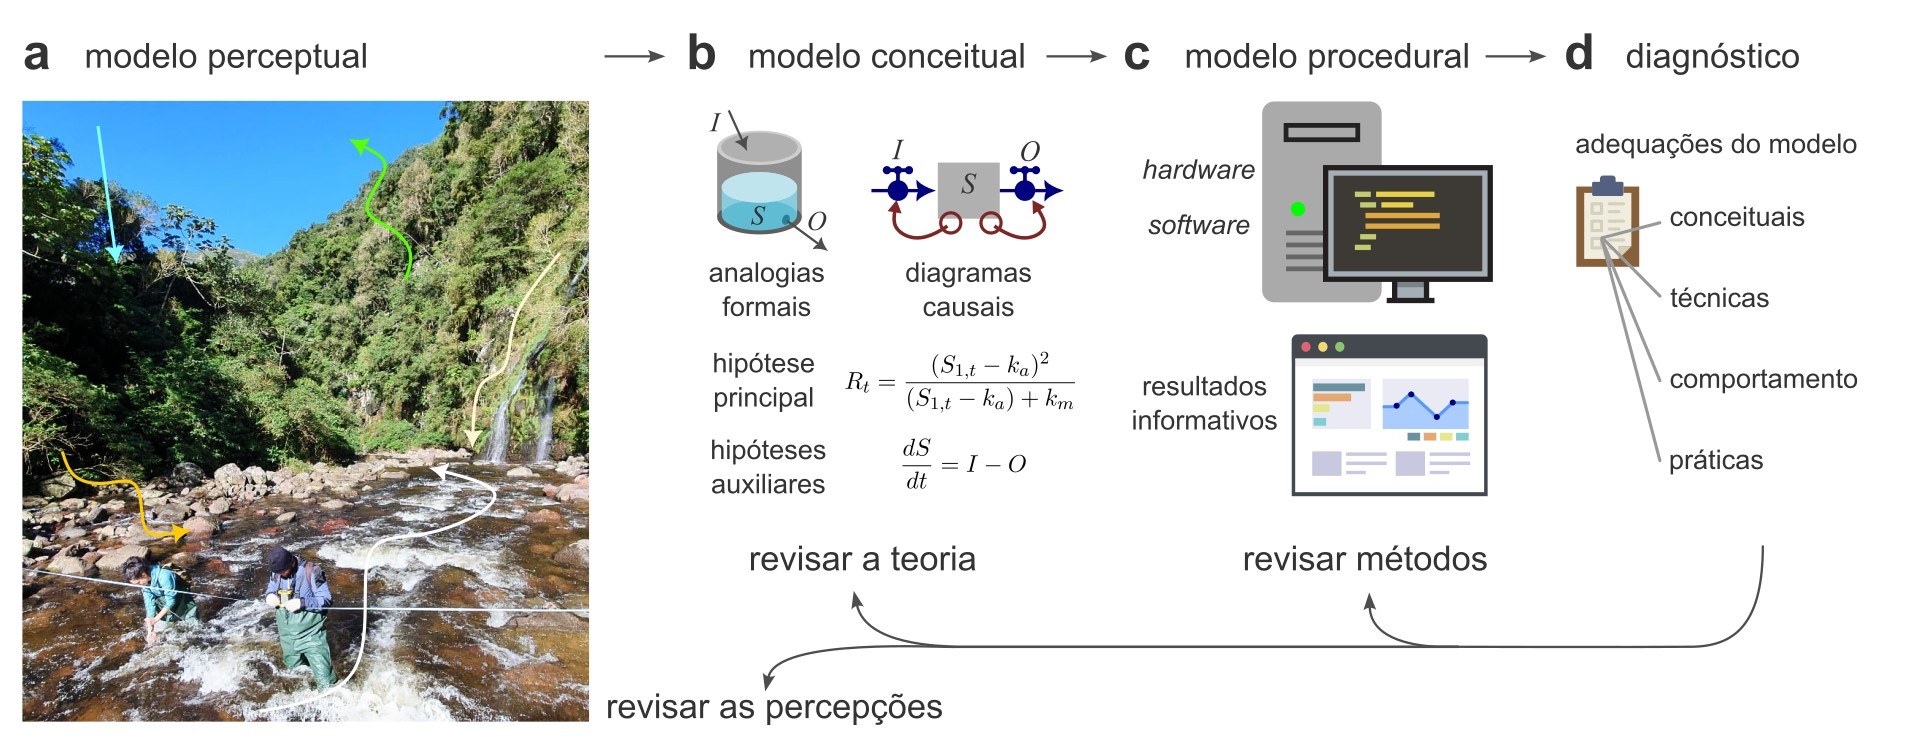
\includegraphics[width=0.95\linewidth]{figs/fig_modelprocess.jpg}		
	\caption[O processo de modelagem]
	{\textbf{---\;O processo de modelagem.}
        A modelagem hidrológica pode ser entendida como um processo iterativo de aprendizado. \;\textbf{a}\;---\;O primeiro estágio consiste no modelo perceptual (modelo mental), que é uma coleção das percepções subjetivas e pessoais adquiridas pela experiência empírica (expedições de campo) e teórica (livros-texto, palestras, aulas, etc). \;\textbf{b}\;---\;O segundo estágio consiste no modelo conceitual, que instancia analogias formais (matemáticas) e diagramas causais (estruturas) para se obter uma hipótese principal objetiva na forma de equações. Diversas hipóteses auxiliares em geral são necessárias, fazendo do modelo conceitual um sistema logicamente aberto (subdeterminado).\;\textbf{c}\;---\;O terceiro estágio consiste no modelo procedural, que é a síntese dos métodos computacionais utilizados (\textit{hardware} e \textit{software}) para simular o modelo conceitual e se obter resultados na forma simbólica de tabelas, gráficos, mapas, animações, etc.\;\textbf{d}\;---\;Por fim, o estágio de diagnóstico aplica diversos procedimentos para avaliar a adequação dos modelos em termos conceituais (problemas teóricos), técnicos (problemas computacionais), comportamentais (justificação empírica) e práticos (impactos na tomada de decisão). O diagnóstico é iterativo, revisando todos os modelos criados, fechando o ciclo de aprendizado. A fotografia em (\textbf{a}) foi gentilmente cedida pela hidróloga Marina Fagundes, que figura medindo a vazão de um rio montanhoso durante uma expedição de campo, Rio Grande do Sul, Brasil.\;
	}
\label{fig:sys:process}  % use qualitative label			
\end{figure}

\begin{adjustwidth}{100pt}{0pt}
\medskip
\small Nossos modelos geralmente têm uma forte congruência com o mundo. É por isso que somos uma espécie tão bem-sucedida na biosfera. Especialmente complexos e sofisticados são os modelos mentais que desenvolvemos a partir da experiência direta e íntima da natureza, das pessoas e das organizações ao nosso redor. No entanto, e ao contrário, nossos modelos estão longe de representar completamente o mundo. É por isso que cometemos erros e somos regularmente surpreendidos. Em nossas cabeças, só conseguimos acompanhar algumas poucas variáveis de cada vez. Frequentemente tiramos conclusões ilógicas de premissas corretas, ou conclusões lógicas de premissas incorretas\footnote{Tradução livre de: \say{\textit{Our models usually have a strong congruence with the world. That is why we are such a successful species in the biosphere. Especially complex and sophisticated are the mental models we develop from direct, intimate experience of nature, people, and organizations immediately around us. However, and conversely, our models fall far short of representing the world fully. That is why we make mistakes and why we are regularly surprised. In our heads, we can keep track of only a few variables at one time. We often draw illogical conclusions from accurate assumptions, or logical conclusions from inaccurate assumptions.}}} -- Donella Meadows \cite{meadows2008}.
\medskip
\end{adjustwidth}

\noindent Seja qual for a posição de Meadows diante das correntes filosóficas, sua visão é clara na direção de que a modelagem é um \textit{processo} que se inicia de forma \textit{subjetiva e pessoal} com modelos mentais, e então vai tornando-se cada vez mais \textit{objetiva e impessoal} a partir de textos, equações e programas de computador. 

\par No âmbito da hidrologia, Keith Beven salienta a perspectiva de Meadows, propondo que o processo de modelagem apresenta pelo menos três estágios representados por modelos de diferentes naturezas: o estágio \textit{perceptual}, o estágio \textit{conceitual} e o estágio \textit{procedural}\footnote{Outros dois estágios adicionais no processo de modelagem incluem a calibração e a validação do modelo procedural, mas esses estágio não são modelos em si, e sim etapas de justificação empírica.} \cite{beven2011}. A Figura \ref{fig:sys:process} ilustra essa concepção, incluindo um último estágio de diagnóstico. O \gls{percept-model} inicia-se com a compreensão subjetiva e qualitativa da hidróloga sobre como uma bacia hidrográfica responde ao eventos de precipitação. Este modelo é profundamente influenciado pelas vivências individuais, estudos, dados analisados e a experiência de campo da hidróloga. É um modelo inerentemente pessoal e varia substancialmente de uma pessoa para outra. Seguindo para o \gls{concept-model}, Beven descreve uma transição para uma representação mais formalizada e simplificada dos processos identificados no modelo perceptual. Este modelo envolve a criação de hipóteses e a adoção de suposições para \textit{abstrair} os processos complexos da realidade de forma palpável e objetiva, frequentemente utilizando-se de formulações matemáticas. Finalmente, o \gls{proced-model} representa a implementação prática do modelo conceitual em um programa de computador. Neste estágio, as equações e conceitos do modelo conceitual são traduzidos em código, permitindo simulações e previsões de fluxos e níveis baseadas em dados de entrada a partir da aplicação de tensões em circuitos eletrônicos. No caso de computadores digitais, este processo envolve a aplicação de métodos numéricos e pode introduzir erros ou aproximações adicionais, tornando a precisão e o cuidado na sua execução extremamente importantes. São essas computações eletrônicas que produzem os resultados supostamente informativos que vemos a partir de tabelas, gráficos, mapas, etc. Para Beven, a interação e a evolução entre esses três modelos são cruciais no processo de modelagem em hidrologia. Com diversas ressalvas, ele inclui mais dois estágios, que seriam a \textit{calibração} e a \textit{validação} do modelo diante de evidências empíricas.  Esses são jargões do realismo pragmático. Uma nomenclatura instrumentalista seria o \textit{condicionamento} e o \textit{teste} diante de evidências empíricas. De uma forma ou de outra, um estágio final de \textbf{diagnóstico} deve conduzir à revisão e refinamento dos modelos elaborados anteriormente, fazendo surgir um \textit{ciclo iterativo de aprendizado} e eventuais \textit{revoluções científicas} na compreensão dos processos hidrológicos.

\par É com essa perspectiva que o objetivo deste capítulo é estabelecer os detalhamentos necessários sobre o processo de modelagem para podermos em breve discutir modelos hidrológicos propriamente ditos. Em determinado ponto do capítulo anterior, tornou-se essencial definir um modelo como um \textbf{veículo simbólico de uma teoria}, uma concepção tipicamente instrumentalista que dialoga com a visão de Nancy Cartwright [>>:cite] -- o que é eficaz na articulação dos problemas epistemológicos que existem por trás das práticas de modelagem. Nessa perspectiva, os modelos são vistos como meros tradutores das nossas teorias ou hipóteses sobre fenômenos reais, como o ciclo hidrológico. No entanto, essa ainda é uma definição genérica e abstrata, que não fornece um entendimento concreto sobre a natureza exata dos modelos. Como enfatizado no início do primeiro capítulo, os modelos hidrológicos surgem materializados nos estados de circuitos eletrônicos de computadores digitais, mas também eles são outras coisas antes dessa materialização. Para articular o enigma do que exatamente são modelos, o presente capítulo vai abandonar o domínio da Epistemologia e da Filosofia da Ciência, adentrando no campo da Ontologia de modelos. Tratarei do problema da representação, do paradigma dos sistemas, da Dinâmica de Sistemas e do diagnóstico de modelos. Se no capítulo anterior estávamos em um terreno com vista panorâmica e ar rarefeito, como no alto de uma montanha, agora certamente estaremos descendo das alturas, seguindo os vales dos riachos. A analogia continua sendo interessante, pois caminho ainda é difícil e íngreme, mas a paisagem é cada vez mais familiar. Cresce a esperança de em breve se estar em um terreno suave e aberto.

\section{Representação} \label{sec:sys:represent}

\par Os modelos desempenham a função de representação de um \gls{sys-target}. Ou seja, justamente por veicular simbolicamente uma teoria, os modelos buscam reeditar um dado fenômeno ou entidade que supostamente existe e se desenvolve no mundo real. O problema de justificar a correspondência entre o modelo e a realidade foi o assunto do primeiro capítulo. Aqui, no entanto, temos um novo problema: \textit{como é possível criar as representações em si}? A saída para esse \gls{problem-repr} consiste em estabelecer um processo de \gls{idealization} do sistema-alvo aliado com a aplicação de \gls{infer-analog}, isto é, a construção de uma \gls{analogy} entre o sistema-alvo e o modelo. Nessa linha, Mary Hesse propõe que tais analogias se manifestam tanto por \textit{modelos materiais}, estruturas semânticas realizadas por objetos físicos, quanto por \textit{modelos formais}, estruturas sintáticas expressas por equações matemáticas implementadas por programas de computador \cite{hesse2017}.

\par O processo de idealização é a base de toda modelagem e se caracteriza por \textit{simplificações deliberadas}, que tornam o modelo mais palpável e compreensível que o sistema-alvo em si, enfatizando aspectos cruciais enquanto ignora detalhes supostamente menos relevantes. De acordo com R. Frigg e S. Hartmann \cite{sep-models-science}, existem duas formas de idealização, que não são mutuamente excludentes: a \gls{idealiz-arist} e a \gls{idealiz-galil}. No caso da idealização Aristotélica, a chave consiste no processo de \gls{abstraction}, quando se remove todas as supostas superficialidades do sistema-alvo, deixando apenas uma suposta \textit{essência}. Em outras palavras, a abstração objetiva preservar a verdade, ainda que apenas a parte dela que é relevante. Em um modelo hidrológico, por exemplo, o dossel da vegetação geralmente é tido como um único reservatório que intercepta a água da chuva. É claro que cada folha e graveto exerce um papel na interceptação, mas esse processo individual é tido como irrelevante e abstraído como um processo geral que ocorre em todo o dossel. Alan Musgrave, contudo, pondera que a abstração também pode resultar em falsidades, em especial quando se introduzem \gls{neglig-premis}, ou seja, quando se negligencia algum fator causal \textit{sabidamente verdadeiro} \cite{musgrave1981}. Ele traz essa crítica inicialmente para as teorias econômicas neoclássicas, mas também é o caso, por exemplo, quando em modelos hidrológicos se ignora a importância da iluminação solar e o sombreamento do relevo sobre os processos evaporativos. A idealização Galileana, por outro lado, consiste na aplicação de uma distorção controlada experimentalmente, que pode ser incrementalmente revertida na direção do simples para o complexo, do ideal para o real \cite{MCMULLIN1985}. Ou seja, a idealização apresenta um \textit{comportamento assintótico} que, no limite, faz com que o modelo se torne idêntico ao sistema-alvo. A referência a Galileu Galilei (1564-1642) remete aos seus famosos experimentos com planos inclinados, que o levaram a concluir que objetos caem ao mesmo tempo, independentemente de sua massa. Nesse caso, o plano inclinado idealizou a queda livre, permitindo uma melhor compreensão do processo físico. Em modelos hidrológicos, um exemplo desse tipo de idealização é a discretização espacial em unidades de resposta, sub-bacias ou rede de drenagem – quando levada ao extremo de pequenas parcelas se aproxima assintoticamente à bacia hidrográfica.

% figure
\begin{figure}[t!] % place figure in the page
	\centering				
	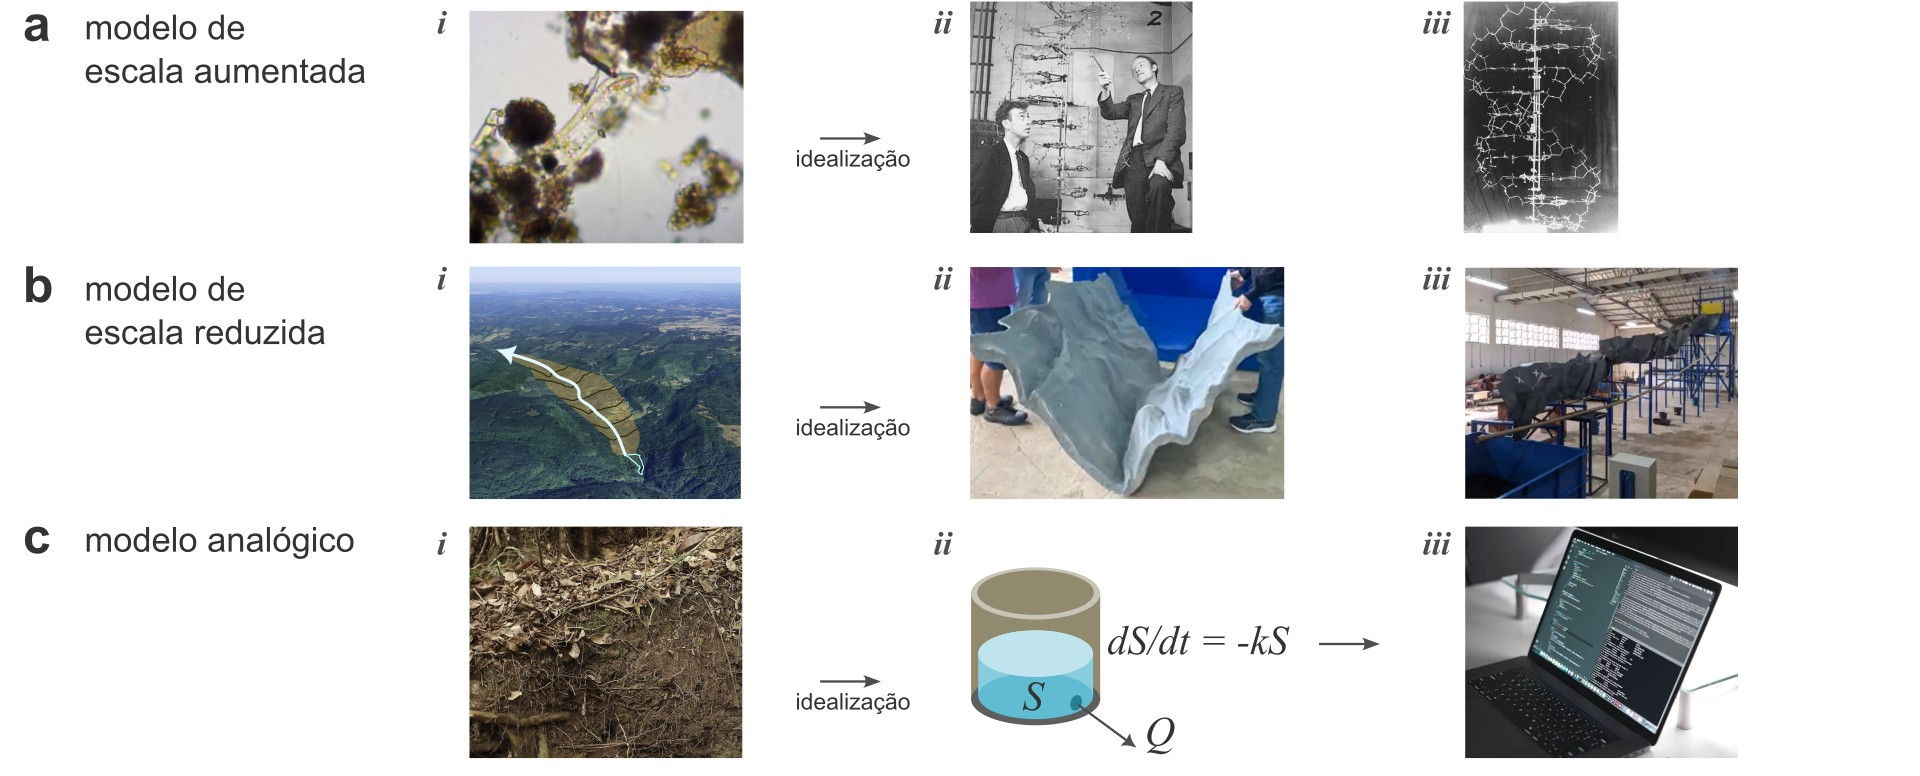
\includegraphics[width=0.95\linewidth]{figs/fig_representation.jpg}		
	\caption[Representação de sistemas por modelos]
	{\textbf{---\;Representação de sistemas por modelos.}
        A idealização é necessária para representar sistemas-alvos em modelos suficientemente tratáveis.\;\textbf{a}\;---\;Um modelo de escala aumentada famoso na Histórica da Ciência foi o modelo da dupla hélice para a molécula de DNA, que armazena o código genético de células orgânicas (detalhe \textrm{\textit{i}}); Francis Crick e James Watson manuseando o modelo (detalhe \textrm{\textit{ii}}); o modelo original de DNA (detalhe \textrm{\textit{iii}}).\;\textbf{b}\;---\;Um modelo de escala reduzida para estudos empíricos de rompimento de barragem. No caso, o modelo representa 5.5 km do vale a jusante da barragem de Canastra, Canela, Rio Grande do Sul (detalhe \textrm{\textit{i}}); a representação topo-batimétrica do vale (detalhe \textrm{\textit{iii}}) com módulos de seções transversais e longarinas de aço, preenchidos com fibra de vidro e resina (detalhe \textrm{\textit{ii}}).\;\textbf{c}\;---\;Um modelo analógico típico da hidrologia para o armazenamento de água no solo e subsolo (detalhe \textrm{\textit{i}}); a analogia formal (homologia) é feita com um reservatório linear, como se fosse um balde com uma saída porosa no fundo (detalhe \textrm{\textit{iii}}); o modelo se realiza em um computador digital, da interação do \textit{hardware} com \textit{software} (detalhe \textrm{\textit{iii}}).\;Créditos das imagens: (\textbf{a}) o autor (detalhe \textrm{\textit{i}}) e de Chadarevian \cite{deChadarevian2003} (detalhes \textrm{\textit{ii}} e \textrm{\textit{iii}}); (\textbf{b}) o autor (detalhe \textrm{\textit{i}}) e Flávia Pereira \cite{Pereira2023} (detalhes \textrm{\textit{ii}} e \textrm{\textit{iii}}); (\textbf{c}) o autor (detalhe \textrm{\textit{i}}) e Pinterest (detalhe \textrm{\textit{iii}}).
	}
\label{fig:sys:represen}  % use qualitative label			
\end{figure}

\par Entre as formas de analogias disponíveis, uma alternativa um tanto direta é construir uma \textit{cópia} daquilo que se entende como sistema-alvo, em uma escala adequada para manipulações por seres humanos. Esses modelos materiais são ditos \gls{scale-models} reduzida ou aumentada, ilustrados na Figura \ref{fig:sys:represen}a e Figura \ref{fig:sys:represen}b. Em certa medida, estamos todos acostumados com modelos desse tipo, pois os brinquedos que manipulamos quando crianças são como modelos em escala reduzida. A maquete de um edifício ou automóvel em um túnel de vento, por exemplo, é um modelo em escala reduzida utilizada para aplicações de engenharia. Átomos de elementos químicos com encaixes para formarem moléculas mais complexas, por outro lado, são modelos em escala aumentada para fins didáticos. Em uma época altamente tecnológica, modelos de escala podem soar como grosseiros ou simplistas, mas na verdade são opções extremamente interessantes para se investigar, visualizar e testar experimentalmente as implicações de uma dada teoria ou hipótese. Um exemplo marcante na História da Ciência que envolveu a contribuição de um modelo de escala aumentada foi a descoberta da estrutura do DNA por Watson e Crick, no início dos anos 1950 \cite{deChadarevian2003}. Apesar da sua atratividade, a \gls{scale-similarity} de representação é viável apenas em casos especiais ou em certas características. Por exemplo, se uma maquete de uma cidade é construída para se observar os efeitos de sombreamento dos edifícios, a redução da escala não interfere nos padrões de sombra produzidos pela luz, pois a geometria é completamente preservada em ambas as escalas. Mas um canal ou tubulação de água em escala reduzida pode manifestar efeitos de viscosidade e tensão superficial muito superiores aos observados na escala real, o que torna a conversão entre as escalas um problema não-trivial. Em problemas de mecânica de fluidos como esse, geralmente a conversão é solucionada por análise dimensional, quando se busca estabelecer uma caracterização do sistema-alvo que é livre de escalas, como o número de Mach, Reynolds e Froude.

\par A depender do sistema-alvo em questão, a representação por modelos de escala reduzida ou aumentada não é possível em razão de algum princípio fundamental ou simplesmente devido à escassez de recursos materiais. Um modelo epidemiológico em escala reduzida evidentemente não é possível por princípios éticos, por exemplo. Já um modelo de escala reduzida de um sistema ambiental, como uma planície de inundação ou a própria atmosfera, pode ser muito caro. Diante dessa condição, é preciso recorrer a uma forma de representação analógica. Em outras palavras, se faz necessário partir de uma abordagem de modelagem que estabelece uma analogia formal, ou \gls{homology}, com o sistema-alvo, ou seja, uma equivalência entre as \textit{estruturas matemáticas} entre o sistema-alvo e o modelo. Na hidrologia isso é frequentemente realizado ao se estabelecer que o solo (ou qualquer outro compartimento do ciclo hidrológico) funciona \textit{como se} fosse um reservatório linear, igual a um balde com um orifício poroso no fundo, como ilustrado na Figura \ref{fig:sys:represen}c. A locução conjuncional \say{como se} é crucial, pois ela que estabelece a analogia que fundamenta a idealização da modelagem. A implementação da analogia formal, isto é, a realização da sua estrutura matemática, em geral acontece a partir da programação de computadores digitais (que é o caso dos modelos hidrológicos), ainda que também seja possível a criação de modelos materiais do sistema análogo. Nesse sentido, os modelos formais deixam muito mais claro do que os modelos de escala a veiculação simbólica da própria teoria ou hipótese sobre o sistema-alvo, pois se está buscando testar uma estrutura matemática a partir de um sistema supostamente análogo. Assim como a dedução, a indução e a abdução, mencionadas no contexto da justificação de teorias do primeiro capítulo, a analogia também consiste em uma forma de inferência, que apresenta a seguinte estrutura lógica \cite{shaw_ashley_1983}:
\begin{enumerate}
    \item Os objetos $O_1, O_2, O_3, ... O_n$ possuem as propriedades $P_2, P_3, P_4, ... P_k$ em comum. 
    \item Os objetos $O_2, O_3, ... O_n$ possuem a propriedade $P_1$ em comum. \\
    \item Portanto, é provável que o objeto $O_1$ possui a propriedade $P_1$.
\end{enumerate}
Com isso, a inferência analógica permite que múltiplos itens sejam avaliados, ainda que em geral se faça a relação entre apenas dois objetos – no caso da modelagem, o sistema-alvo e o modelo. Outra característica é que, ao contrário da abdução, a inferência analógica não é uma forma especial de indução, pois não envolve uma generalização universal a partir de enunciados singulares. Ainda assim, também não é um raciocínio seguro como a dedução, sendo inexistente a garantia da verdade da sentença consequente. Por isso, a inferência analógica é tida como um forma independente de inferência.

\par Em muitos casos de pesquisa e investigação científica, obter uma representação empiricamente adequada de um determinado sistema-alvo não é necessariamente o objetivo final da construção de modelos, mas sim a \textit{exploração} experimental das implicações da teoria que o modelo transmite. Em outras palavras, em vez de confrontar os modelos com evidências empíricas para testar ou confirmar as hipóteses embutidas em sua estrutura, eles também podem cumprir a função epistêmica de \textit{articulação} da própria teoria. Nesse sentido, Axel Gelfert introduz o conceito de \textbf{experimentação exploratória} com modelos, um processo que tem o potencial de revelar várias novas hipóteses e elucidações no campo teórico \cite{gelfert2016}. A vantagem dos \gls{explore-models}, muitas vezes mantidos como \gls{mini-models}\footnote{tradução livre de \textit{toy models}, em inglês.} para facilitar seu entendimento, é que a analogia com o sistema-alvo sugere que comportamentos inesperados e surpreendentes do modelo exploratório possam eventualmente ser observados empiricamente no sistema-alvo, em condições limite. Um exemplo que Axel Gelfert destaca da História da Ciência são os experimentos com o modelo ecológico de Lotka-Volterra, que explorou a dinâmica predador-presa. Embora o modelo não tenha fornecido previsões empiricamente precisas, ele ofereceu vários \textit{insights} qualitativos importantes sobre as interdependências entre diferentes espécies em uma situação de completo isolamento: ficou demonstrado que oscilações nas populações podem emergir mesmo sem interferências externas. No campo ambiental e hidrológico, por exemplo, modelos exploratórios podem contribuir para o entendimento de impactos de \textit{cenários} jamais observados no registro histórico, como as mudanças climáticas em curso atualmente. Nessa concepção, os modelos exploratórios são ferramentas versáteis na pesquisa científica, desempenhando vários papéis, desde fornecer pontos de partida para futuras investigações, demonstrações de \textit{prova de princípio}, elaboração de explicações potenciais e avaliação da adequação do modelo. Além disso, eles são particularmente valiosos em situações em que as teorias estabelecidas estão em crise, permitindo que novos paradigmas possam ser propostos a partir das explorações experimentais.

\section{Sistemas} \label{sec:sys:systems}

\par Quando tratamos de modelos surge um conceito central que é a noção de \gls{system} – afinal, os modelos veiculam uma teoria ao representar um sistema-alvo. Um sistema define-se por \textit{um conjunto de partes com relações entre si}. Essa definição pode parecer singela, mas ela traz consigo uma visão de mundo holística que instancia coisas que transcendem a materialidade. Como já foi salientado, ao explorar a essência das \say{coisas}, ingressamos no campo da \textbf{Ontologia}, que é o estudo daquilo que existe. A pergunta ontológica é: \textit{o que existe}? Consideremos, por exemplo, uma questão ontológica clássica: a existência de cadeiras \cite{bradley2019}. Se cadeiras existem ou não, a resposta varia conforme a interpretação sobre a natureza dos elementos fundamentais. Sob um enfoque reducionista, que considera os átomos de matéria como as únicas entidades possíveis, as cadeiras são meros conjuntos de átomos e, portanto, \textit{não existem}. Essa perspectiva, que vai de baixo para cima, leva a uma conclusão inquietante: nada existe, \textit{nem mesmo pessoas}, exceto matéria sendo dispersada em um grande fluxo do nada para o nada. Contudo, é evidente que as cadeiras existem; do contrário, estaríamos todos sentados no chão. Mais evidente ainda é o fato de existirem pessoas, do contrário eu não poderia escrever este texto e ninguém poderia o ler. A solução para instanciar a existência de objetos como cadeiras ou pessoas consiste em ter um enfoque holístico, ou seja, uma visão de cima para baixo. Essa perspectiva compreende objetos e sujeitos como entidades que \textbf{emergem} da relação e interação entre os seus componentes fundamentais, seus elementos, suas partes. Nesse sentido, uma cadeira existe independente de seu material, seja ele metal, madeira ou plástico. Ao mesmo tempo, não adianta obter um amontoado de madeira e esperar que dali surja uma cadeira: é necessário \textbf{organização}. Uma cadeira seria então o sistema que emerge a partir de uma estrutura organizada que cumpre a função de servir de assento.

\par As raízes do pensamento sistêmico remontam à Antiguidade, em especial nas ideias de Aristóteles (384-322 a.C.). Esse filósofo grego desenvolveu um conceito denominado de \gls{hilomorphism}, que permeia diversos aspectos de sua filosofia, abrangendo desde a ciência natural até a política. Com essa perspectiva, Aristóteles defendia que todo objeto existente é composto tanto de \textbf{matéria} quanto de \textbf{forma}, sendo esta última essencial para a \textit{unificação} do objeto em uma entidade [>>:cite]. Por exemplo, em organismos vivos, o corpo representa a matéria e a alma, a forma. Na política, os cidadãos seriam a matéria e a constituição, a forma. Com o advento do método científico na modernidade, principalmente influenciado pelas ideias de Descartes, houve um declínio na concepção da forma como unificadora ontológica. No seu \textit{Discurso do Método}, Descartes introduziu uma abordagem analítica, reducionista e mecanicista do mundo. Por exemplo, um dos passos essenciais de seu método para dissipar dúvidas envolve o isolamento das dificuldades em quantas partes forem necessárias para uma resolução mais fácil, construindo a visão completa do todo gradativamente, do mais simples para o mais complexo. Nesse rumo, o foco deve ser mantido nas partes individuais, sendo o todo uma mera sobreposição ou concatenação linear. Paira aqui um \textbf{princípio da aditividade}, que permite o entendimento das escalas maiores a partir das escalas menores. Descartes ilustra essa essa visão ao descrever o coração humano nos termos de um bomba hidráulica que apresenta a função de distribuir o sangue, sugerindo que o corpo humano é na verdade uma máquina, com cada órgão exercendo uma função específica. Esse movimento ganhou tração a partir da física de Newton, sendo um marco de seu apogeu a mecânica celeste de Laplace e mais tarde, no século XIX, a termodinâmica clássica, que estabeleceu leis cegas e implacáveis que descrevem a complexidade aleatória e desorganizada.

\par O renascimento do pensamento sistêmico no século XX foi marcado substancialmente pela obra do biólogo Ludwig von Bertalanffy (1901-1972). Criticando o paradigma mecanicista e reducionista hegemônico, Bertalanffy iniciou a \textbf{Teoria Geral dos Sistemas} a partir da década de 1920, ainda que ela tenha se consolidado somente na década de 1960. A influência da biologia nesse movimento contemporâneo do pensamento sistêmico esteve parcialmente relacionada com a refutação das teorias vitalistas sobre os organismos vivos. Dado que os seres vivos são completamente compostos da mesma matéria que o seu ambiente, surgiu a necessidade de explicar o enigma de como simples moléculas podem formar células, tecidos, órgãos, indivíduos e sociedades. Mas também ocorreram influências de outras teorias e disciplinas da época, como a cibernética e a teoria da informação, que introduziram os conceitos de \gls{feedback} e sinais entre os componentes de um sistema. A generalidade da teoria reside no que Bertalanffy chama de \gls{struc-iso}, que é a analogia formal (homologia) entre fenômenos completamente diferentes em termos materiais, mas que apresentam as mesmas relações entre as partes, ou seja, a mesma forma. Nesse sentido, a proposta torna-se um tanto ambiciosa, pois Bertalanffy sugere que há um potencial unificador para uma Ciência que estava demasiadamente compartimentalizada:
\begin{adjustwidth}{100pt}{0pt}
\medskip
\small O ponto de vista sistêmico penetrou e provou ser indispensável numa grande variedade de campos científicos e tecnológicos. Esse o fato ulterior de que ele representa um paradigma original no pensamento científico (para usar a expressão de Thomas Kuhn) tem como consequência que o conceito de sistema pode ser definido e desenvolvido de diferentes formas como requerido pelos objetivos de pesquisa. -- Ludwig von Bertalanffy \cite{bertalanffy}.
\medskip
\end{adjustwidth}

\par A teoria de Bertalanffy, em essência, defende uma compreensão holística dos organismos vivos e dos sistemas em geral, tratando-os como \gls{sys-open} que interagem constantemente com o ambiente e estão sujeitos ao fluxo de matéria, energia e informação. Esta visão contrasta com a perspectiva colocada pela termodinâmica clássica, focada em sistemas fechados regidos pela desorganização aleatória. Sistemas abertos, por outro lado, permitem a emergência de homeostase, metabolismo e estado estacionário, fenômenos que, segundo Bertalanffy, ajudam a explicar as aparentes violações das leis da termodinâmica na biologia. Na visão mecanicista do mundo, o destino de qualquer sistema é rigidamente determinado por leis cegas e pelas suas condições iniciais. Mas Bertalanffy destaca que isso não ocorre em sistemas abertos, exemplificando com o fenômeno da equifinalidade\footnote{Keith Beven adotou o termo \say{equifinalidade} para descrever o problema da subdeterminação em modelos hidrológicos a partir da Teoria Geral dos Sistemas de Bertalanffy [>>:cite].}, que ocorre quando diferentes condições iniciais levam ao mesmo estado final, um processo observado principalmente no desenvolvimento embrionário de organismos vivos. A própria evolução darwiniana, Bertalanffy aponta, também aparentemente viola os ditames da segunda lei da termodinâmica, pois ela propicia um acúmulo de informação e complexidade ao longo do tempo. É claro que as leis da termodinâmica não são violadas em nenhum dos casos, mas é a capacidade de importação de energia livre a partir de fontes em degradação que permite os sistemas abertos a se conservar estáveis contra o fluxo natural da desordem, em um processo de constante \textit{auto-organização}.

\par Ainda que Bertalanffy admita que a Teoria Geral dos Sistemas possa ser aplicada de forma abrangente a partir do ele denominou de \textit{modelos verbais}, ele ilustra que \textit{modelos formais} de sistemas podem ser derivados a partir de uma formulação matemática mais ou menos geral. No caso, essa formulação envolve um sistema de equações diferenciais simultâneas. Assim, para $n$ elementos caracterizados por uma medida quantitativa $S$:

\begin{linenomath*}
\begin{equation}
\label{eq:systems}
\begin{split}
    \frac{dS_1}{dt} &= f(S_1, S_2, ..., S_n)\\
    \frac{dS_2}{dt} &= f(S_1, S_2, ..., S_n)\\
    ...\\
    \frac{dS_n}{dt} &= f(S_1, S_2, ..., S_n)\\
\end{split}
\end{equation}
\end{linenomath*}
Ou seja, qualquer variação em $S_i$ é uma função do estado geral do sistema, o que inclui todos os outros elementos. Essa formulação também possibilita a destruição da relação entre as partes: basta fazer com que o estado $S$ de um elemento seja apenas uma função de si mesmo, isto é,  $dS_i/dt = f(S_i)$. Nesse caso, o sistema como entidade ontológica deixa de existir, sendo então o estado final do todo completamente reduzido à sobreposição dos estados dos elementos individuais. Mas quando existem relações, por mais triviais que sejam, Bertalanffy demonstra que das equações diferenciais emergem uma rica variedade de \textit{comportamentos finais}, como o crescimento ou decaimento exponencial e os processos descritos pela curva logística, como a saturação e autocatálise. Com apenas dois elementos, o sistema linear de coeficientes constantes assume a seguinte forma geral:
\begin{linenomath*}
\[
\begin{split}
    dS_1/dt &= c_{11}S_1 + c_{12}S_2\\
    dS_2/dt &= c_{21}S_1 + c_{22}S_2\\
\end{split}
\]
\end{linenomath*}
Nesse sistema simples, a expansão por série de Taylor permite que soluções sejam obtidas para $S_1$ e $S_2$ via análise matemática. As diferentes soluções demonstram a emergência de diferentes \textbf{condições de estabilidade} (Figura \ref{fig:sys:systems}\,a). Isso pode ser visualizado graficamente a partir de um \textbf{plano de fase} em que as trajetórias dos estados dos dois elementos são desenhadas e também pela evolução das variáveis no domínio temporal. Assim, as múltiplas configurações de valores dos parâmetros (coeficientes) e também das condições iniciais revelam os \gls{atractors} que atuam sobre o sistema. Por exemplo, em certas condições o sistema é estável e migra de uma \textit{fonte} para um estado final ($S^*_1, S^*_2$), ou nó, em um \textit{ralo}. Isso pode ocorrer suavemente ou por \textbf{oscilações amortecidas} (Figura \ref{fig:sys:systems}\,b, detalhes \textrm{\textit{i}} e \textrm{\textit{ii}}). Em outras condições o sistema é instável, migrando eternamente, seja em uma direção fixa ($-\infty$ ou $+\infty$) ou em \textbf{oscilações amplificadas} (Figura \ref{fig:sys:systems}\,c, detalhes \textrm{\textit{i}} e \textrm{\textit{ii}}). De outra forma, o sistema pode apresentar \textbf{oscilações estáveis}, permanecendo eternamente em um laço quando visualizado no plano de fase (Figura \ref{fig:sys:systems}\,b, detalhe \textrm{\textit{iii}}). Um exemplo famoso de oscilações estáveis é o sistema não-linear de Lotka-Volterra mencionado na Seção \ref{sec:sys:represent}, que simula a interação entre a populações de presas $S_1$ e a população de predadores $S_2$:
\begin{linenomath*}
\[
\begin{split}
    dS_1/dt &= r_{1}S_1 - c_{1}S_1S_2\\
    dS_2/dt &= -r_{2}S_2 + c_{2}S_1S_2\\
\end{split}
\]
\end{linenomath*}
Em que $r_1$ e $r_2$ são taxas de crescimento e decaimento, respectivamente. O produto $S_1S_2$ busca representar a taxa de encontros entre presas e predadores, ponderados pelos coeficientes $c_1$ e $c_2$, criando uma retroação que equilibra as populações em ciclos. Bertalanffy salienta que esses são exemplos simples que ajudam a ilustrar a versatilidade dos sistemas em representar os padrões observados na natureza. Se o sistema de interesse possui diversas relações ou mesmo complexidades maiores, como termos parciais, a solução analítica do modelo pode ser extremamente difícil ou até impossível, restando aplicar métodos numéricos para resolver as equações em um domínio qualquer, seja no tempo ou no espaço (ou ambos).

% figure
\begin{figure}[t!] % place figure in the page
	\centering				
	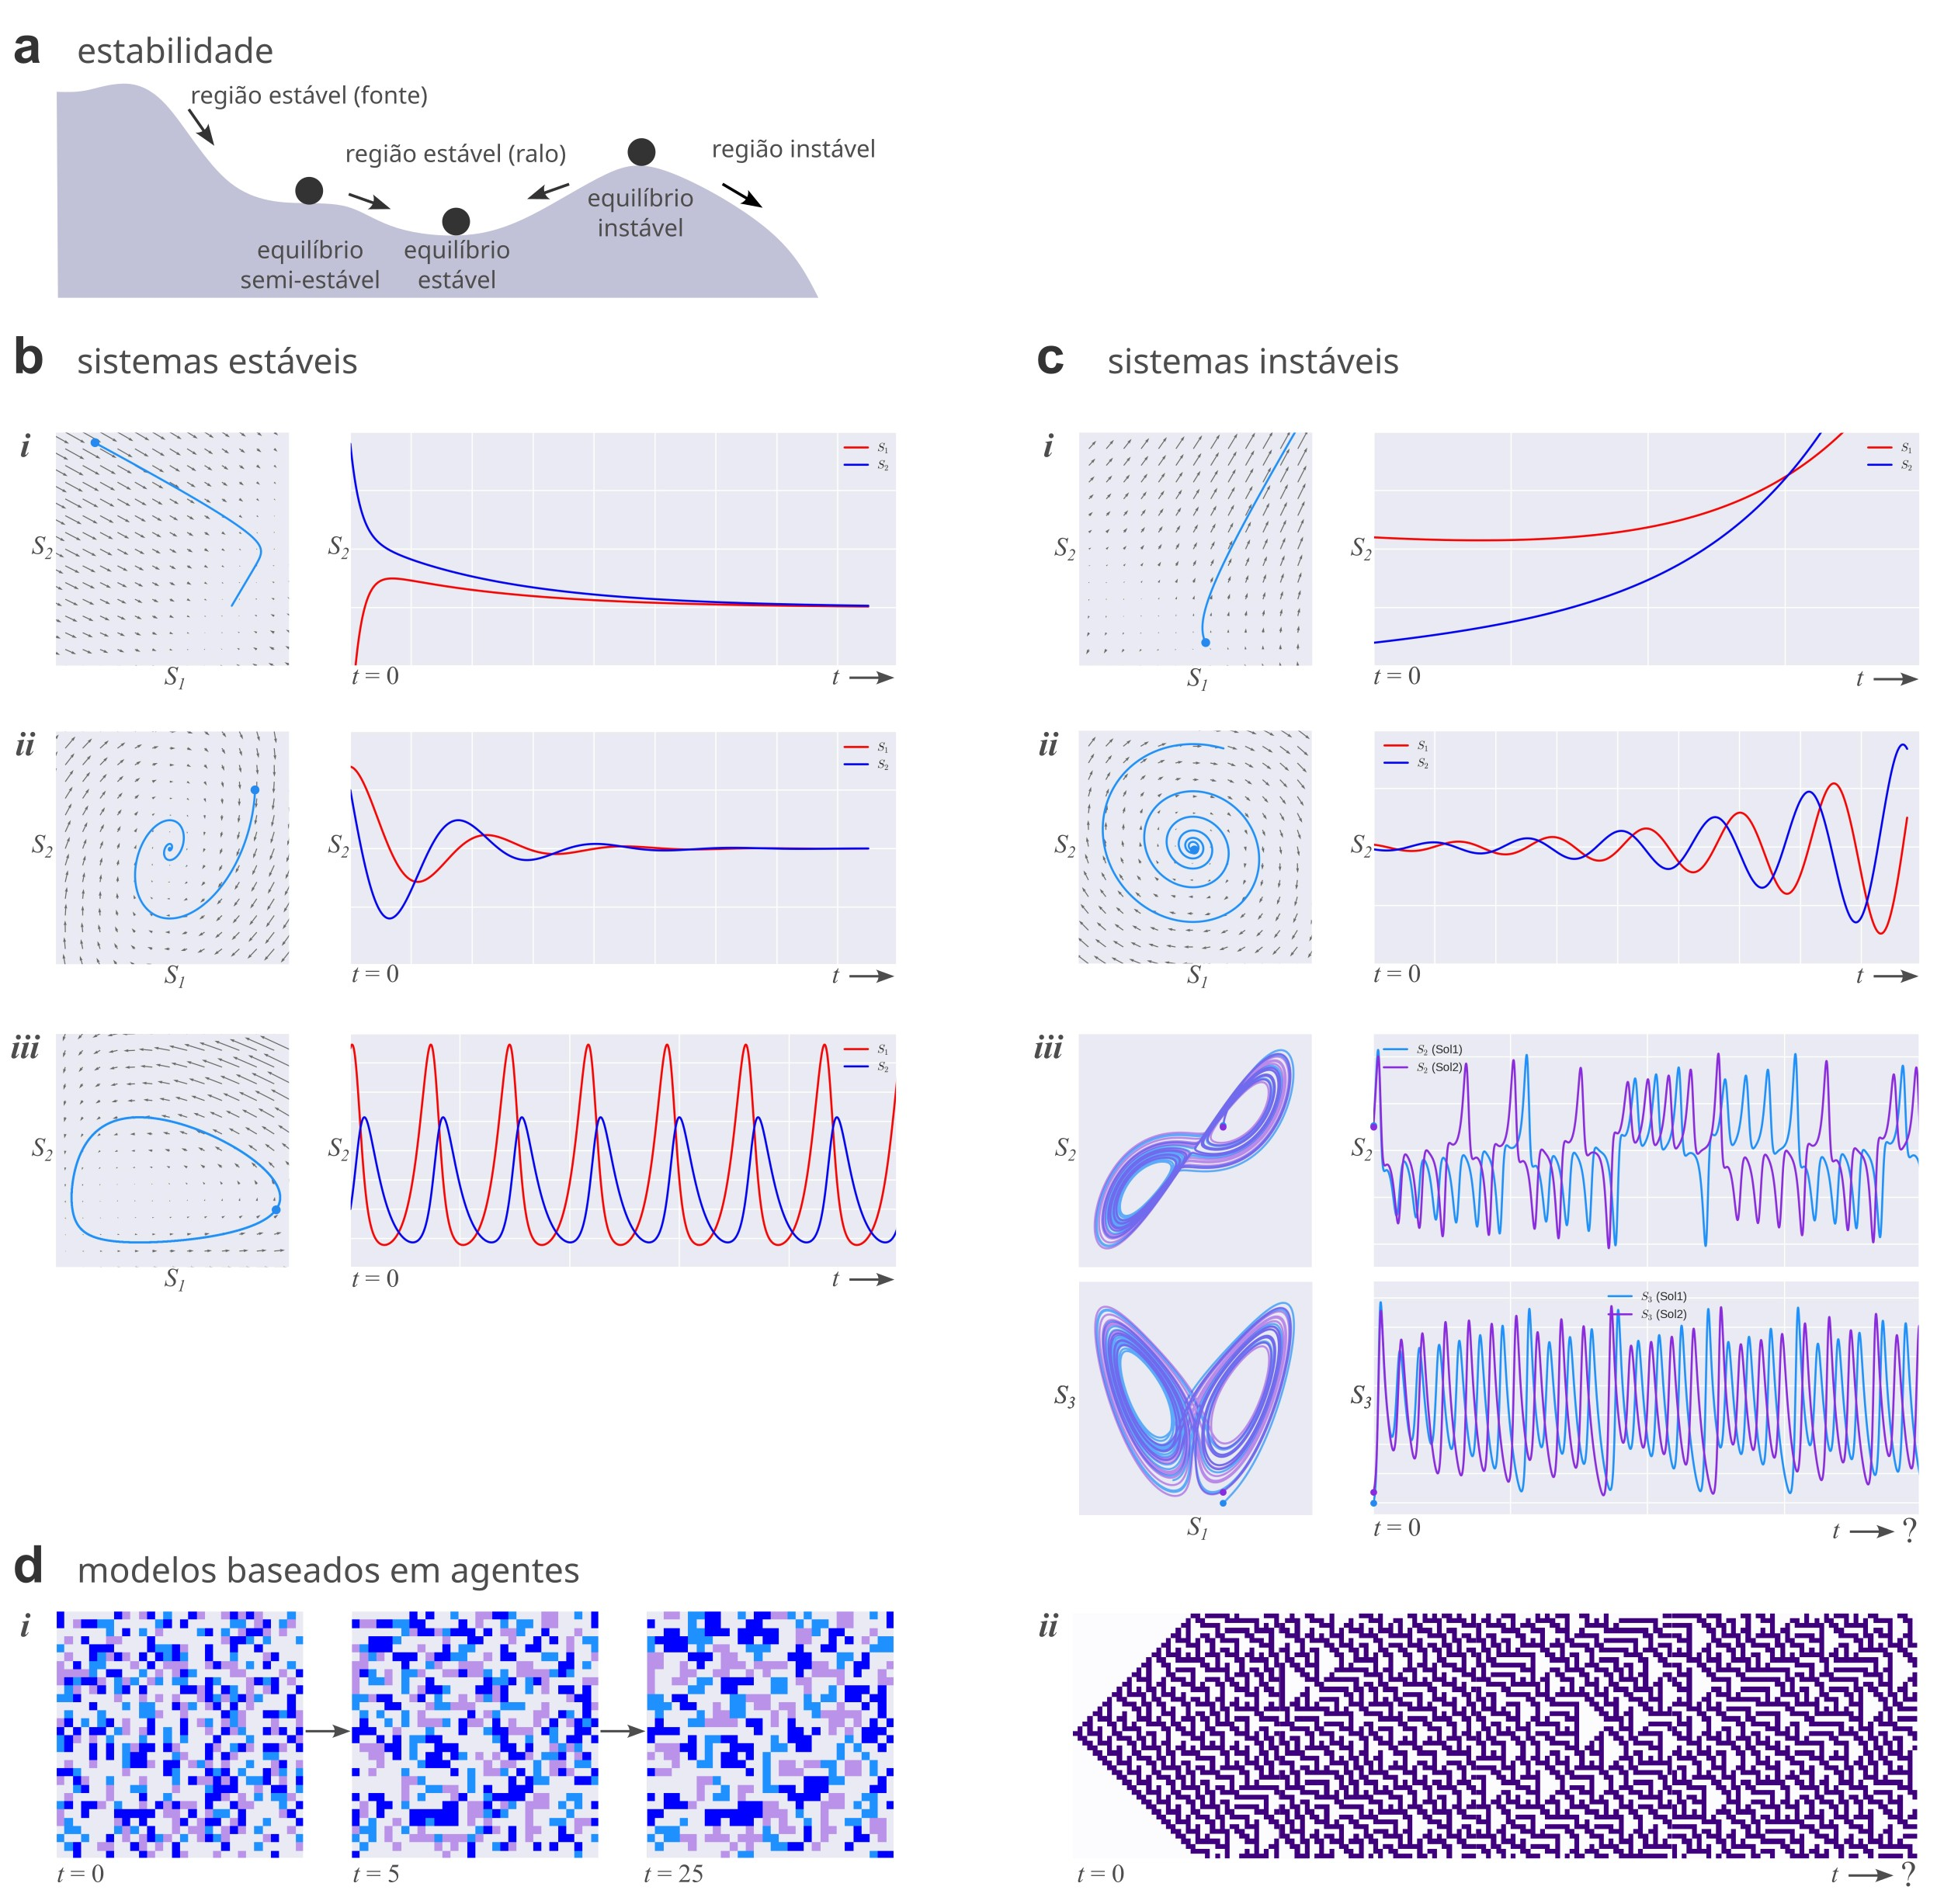
\includegraphics[width=0.95\linewidth]{figs/fig_systems.jpg}		
	\caption[Estabilidade de sistemas]
	{\textbf{---\;Estabilidade e comportamento de sistemas.} Um sistema define-se por um conjunto de partes com relações entre si. Como são as relações que unificam o todo, comportamentos finais similares emergem em diferentes campos científicos.\;\textbf{a}\;---\;O comportamento de um sistema pode ser classificado em estável ou instável, a depender das suas condições iniciais e de contorno. \;\textbf{b}\;---\;Sistemas estáveis com dois elementos ($S_1$ e $S_2$): decaimento exponencial (detalhe \textrm{\textit{i}}) e oscilações amortecidas (detalhe \textrm{\textit{ii}}) fazem um movimento assintótico em direção a um ponto de equilíbrio, sendo variações do sistema linear homogêneo. Um sistema estável também pode assumir oscilações eternas em torno do ponto de equilíbrio, como no caso do modelo presa-predador de Lotka-Volterra, um sistema não-linear (detalhe \textrm{\textit{iii}}). \;\textbf{c}\;---\;Sistemas instáveis com dois elementos ($S_1$ e $S_2$): crescimento exponencial (detalhe \textrm{\textit{i}}) e oscilações amplificadas (detalhe \textrm{\textit{ii}}) fazem um movimento em direção a $+\infty$ ou $-\infty$ (ou ambos), sendo também variações do sistema linear homogêneo. A instabilidade também pode ser caótica, como no modelo de Lorenz, um sistema não-linear com três elementos ($S_1$, $S_2$ e $S_3$; detalhe \textrm{\textit{iii}}). No caso do sistema caótico, duas soluções (em azul e roxo) são visualizadas para condições iniciais muito próximas, mas que divergem no longo prazo (alta sensibilidade às condições iniciais).\;\textbf{d}\;---\;Modelos baseados em agentes ilustram que comportamentos complexos podem emergir a partir de interações simples nas vizinhanças imediatas de cada agente. O modelo de Schelling (detalhe \textrm{\textit{i}}) ilustra o surgimento de agrupamentos ordenados a partir de condições iniciais aleatórias. A Regra 30 de Wolfram (detalhe \textrm{\textit{i}}) ilustra a irredutibilidade computacional: o único jeito de entender o comportamento final do sistema é simular o modelo passo-a-passo. 
	}
\label{fig:sys:systems}  % use qualitative label			
\end{figure}

\par Antes de avançarmos para tópicos mais práticos relacionados a modelos hidrológicos e sistemas ambientais, é essencial destacar dois importantes desenvolvimentos teóricos que emergiram na segunda metade do século XX, influenciados pela Teoria Geral dos Sistemas. O primeiro é a descoberta do \gls{chaos}, que caracteriza alguns modelos de sistemas não-lineares. O segundo é a identificação do \gls{problem-irred}. No que diz respeito ao caos determinístico, essa descoberta origina-se da \textit{sensibilidade} extrema de certos sistemas não-lineares às condições iniciais. Esta sensibilidade é exacerbada quando sistemas são implementados em computadores digitais. Devido ao \gls{round-error} inerente à representação numérica, distorções tendem a se amplificar a cada passo computacional, afetando substancialmente os resultados das simulações. Este efeito foi observado acidentalmente por Edward Lorenz em 1959, através de simulações atmosféricas que deveriam ser idênticas [>>:cite]. Porém, uma delas utilizou valores arredondados para as condições iniciais. Essa pequena alteração nos valores iniciais provocou mudanças drásticas no estado final do sistema climático simulado, originando o termo \say{efeito borboleta} – a sugestão de que o bater de asas de uma borboleta eventualmente cause uma tempestade em outro lugar do planeta. Para o caso o modelo atmosférico, Lorenz reduziu o fenômeno caótico em um sistema não-linear com três elementos:
\begin{linenomath*}
\[
\begin{split}
    dS_1/dt &= \sigma (S_2 - S_1)\\
    dS_2/dt &= rS_1 - S_2 + S_1S_3\\
    dS_3/dt &= -bS_3 + S_1S_2\\
\end{split}
\]
\end{linenomath*}
Em que $\sigma$, $r$ e $b$ são parâmetros constantes. O \gls{strange-atrc} desse sistema é ilustrado em dois planos de fase na Figura \ref{fig:sys:systems}c, no detalhe \textrm{\textit{iii}}. O detalhe também ilustra duas trajetórias que se iniciaram muito próximas, mas que assumem comportamentos diferentes no longo prazo. Por outro lado, o problema da irredutibilidade computacional relaciona-se (principalmente) com a aplicação de \gls{abm-models}. Os modelos baseados em agentes representam sistemas por meio de elementos fundamentais – os agentes – que seguem regras simples em sua vizinhança imediata. Quando representados em uma matriz regular, como em um tabuleiro, esses modelos são chamados de \textbf{autômatos celulares}. Um modelo de agentes exemplar é o \textbf{modelo de segregação de Schelling} [>>:cite]. Nesse modelo, os agentes possuem categorias qualitativas. A cada passo de tempo os agentes avaliam a sua vizinhança imediata e decidem se vão se mudar de lugar ou ficar ali mesmo, a depender da sua taxa de tolerância com agentes de categorias diferentes. Esse sistema com regras simples faz emergir espontaneamente agrupamentos organizados, como ilustrado na Figura \ref{fig:sys:systems}d, detalhe \textrm{\textit{i}}. Nessa linha, Stephen Wolfram demonstra que regras simples em determinados sistemas podem gerar uma complexidade imprevisível, acessível apenas por meio de simulações que avaliam o sistema \textit{passo-a-passo} [>>:cite]. Essa lei computacional surgiu a partir de experimentos com autômatos celulares que seguiam regras simples de conversão booleana (de 0 para 1 e vice-versa) baseadas na representação binária. Algumas regras, como a \textbf{Regra 30}, apresentam irredutibilidade computacional (Figura \ref{fig:sys:systems}d, detalhe \textrm{\textit{ii}}). Tanto o caos determinístico quanto a irredutibilidade computacional transmitem a mesma mensagem: são questões que lançam dúvidas sobre a \textit{capacidade preditiva} de teorias em se tratando de sistemas dinâmicos e não-lineares. Ao mesmo tempo, são conceitos que reforçam a importância da adequação empírica e estimativa de incertezas epistêmicas para que políticas sejam baseadas em \textit{evidências}, não apenas em \textit{teorias}, como foi explorado no capítulo anterior.

\section{Dinâmica} \label{sec:sys:dynamics}

\par O advento do paradigma sistêmico, na década de 1960, possibilitou o surgimento da disciplina da \gls{sys-dyn}, que é, na verdade, uma fusão da engenharia de controle com a ciência da gestão e da tomada de decisão. A Dinâmica de Sistemas, como o nome indica, estuda a evolução de sistemas complexos ao longo do tempo. Além disso, John Sterman defende que a Dinâmica de Sistemas é fundamentalmente um método para \textit{aprender} sobre o comportamento de sistemas complexos \cite{sterman2000}. Como salientado na segunda epígrafe deste capítulo, Sterman defende que os modelos permitem, em última instância, ganhar \textit{insights} sobre a estrutura e o comportamento dos sistemas, explorando \gls{leverage-pts}\footnote{Tradução livre de \textit{leveraing points}, em inglês.} para obter resultados desejados na formulação de políticas e na tomada de decisões. A capacidade de um modelo prever precisamente o estado de um dado sistema, por essa perspectiva, não é tão importante quanto compreender o seu funcionamento e elaborar estratégias de ação. A criação desta disciplina é atribuída a Jay Forrester (1918 - 2016), que buscava entender o comportamento de sistemas sob uma perspectiva tecnológica e gerencial, ou seja, focada na solução de problemas e na conquista de objetivos pré-estabelecidos, desde se obter uma fatia do mercado por uma indústria até se reduzir a concentração de gases de efeito estufa na atmosfera. Isso é ilustrado pelo seu relato de que as ideias fundamentais sobre esta disciplina manifestaram-se a partir de um desafiador problema industrial na \textit{General Eletrics}, relacionado a oscilações de longo prazo em postos de trabalho. Após estudar os processos de tomada de decisão da indústria, ele utilizou uma simulação simples, com lápis e papel, que revelou um potencial de oscilações na própria organização interna do sistema:

\begin{adjustwidth}{100pt}{0pt}
\medskip
\small Mesmo com a constante entrada de pedidos, haveria instabilidade no emprego como consequência das políticas de tomada de decisão comumente usadas na cadeia de suprimentos. Esse primeiro sistema de controle de inventário, com simulação de lápis e papel, foi o início do campo da Dinâmica de Sistemas\footnote{Tradução livre de: \textit{even with constant incoming orders, one would get employment instability as a consequence of commonly used decision-making policies within the supply chain. That first inventory-control system with pencil and paper simulation was the beginning of the system dynamics field}} – Jay Forrester \cite{forrester2007}.
\medskip
\end{adjustwidth}

\noindent Apesar de seu início com lápis e papel, a Dinâmica de Sistemas evidentemente exige o uso de computadores digitais para simular modelos de grande complexidade em contextos industriais, urbanos, sociais, econômicos, ambientais e globais. Um exemplo de aplicação global é o modelo de mundo \texttt{World3}, cujas simulações foram exploradas por Donella Meadows em \textit{Limites do crescimento}, que integrava o grupo de pesquisa de Forrester no MIT. Atualmente, a aplicação dos conceitos e a construção de modelos de Dinâmica de Sistemas são tipicamente realizadas com \textit{softwares} como \texttt{Stella} e \texttt{Vensim}, que utilizam interfaces gráficas avançadas para facilitar a elaboração de sistemas complexos.

\par A Dinâmica de Sistemas formaliza a arquitetura básica observada em modelos hidrológicos e ambientais. Essa arquitetura, em termos filosóficos, é uma ontologia singular que consiste no \gls{compart-models}, ilustrada na Figura \ref{fig:sys:dynamics}a. Na hidrologia, ela corresponde ao modelo de reservatórios ou \say{baldes}. Essa abordagem se consolidou na área ambiental, principalmente devido à facilidade de abstração e à (relativa) baixa demanda computacional. Outro aspecto que contribuiu nesse sentido é que as evidências empíricas sobre processos ambientais frequentemente são resultantes de processos agregados, como a vazão de um rio a ou a concentração de alguma substância na água ou no ar, fato que está mudando com o advento de tecnologias de sensoriamento remoto de alta resolução espacial e temporal. No entanto, Sterman argumenta que os modelos de compartimentos não são a única forma de representação na Dinâmica de Sistemas. Esta também admite arquiteturas com partes desagregadas, heterogêneas ou mesmo individualizadas, como os modelos baseados em agentes mencionados anteriormente \cite{sterman2018}. Diante disso, Sterman estabelece uma atitude pragmática, argumentando que a decisão em torno da arquitetura do modelo deve ser pensada sob o enfoque do problema que se está avaliando, mas sem perder a capacidade manejar o modelo com facilidade. Como exemplo, ele menciona que o modelo epidemiológico SIR\footnote{A sigla SIR deriva de Suscetível, Infeccioso e Recuperado.} é um modelo de compartimentos que exibe praticamente o mesmo comportamento final agregado que qualquer outra versão mais detalhada. A justificativa para introduzir heterogeneidades, como grupos etários, espacialização ou ainda agentes que seguem mais ou menos regras de distanciamento social deve residir nos propósitos finais do estudo, no escopo das recomendações relevantes para a formulação de políticas e tomada de decisão. Do contrário, incorre-se em uma regressão praticamente infinita de detalhamentos: afinal, porque modelar apenas os agentes hospedeiros se é possível modelar os seus órgãos, células e inclusive as próprias bactérias ou vírus? Outra questão relevante em torno da arquitetura detalhada é a sua alta demanda computacional. Ainda que atualmente sejam acessíveis e um tanto sedutoras, Sterman ressalta que as simulações altamente detalhadas com grande tempo de simulação introduzem vieses cognitivos no processo de modelagem, em especial na componente iterativa. No caso, surge uma resistência tanto para revisar aspectos conceituais mais profundos quanto para diagnosticar o modelo a partir de análises de sensibilidade e de incertezas, que exigem muitas simulações.   

\par Na arquitetura de compartimentos, a \gls{causal-struct} do sistema modelado é definida pelo arranjo de compartimentos conectados por fluxos que podem ser materiais (taxas de transferência) ou de informação (laços de retroação positiva e negativa). Pela perspectiva aristotélica, a \textit{matéria} do sistema são os compartimentos, enquanto que a \textit{forma} do sistema são os fluxos. Assim, dois conjuntos idênticos de compartimentos, quando conectados por diferentes fluxos materiais e de informação, revelam-se sistemas completamente diferentes. No jargão da Dinâmica de Sistemas, a ênfase na forma geralmente é expressa pelo fato de que \textit{a estrutura causal de um sistema define o seu comportamento}. O modelo deve ser inicialmente visualizado através de um \gls{causal-diag}, como mostrado na Figura \ref{fig:sys:dynamics}a. Aqui, é crucial estabelecer adequadamente a \gls{bounds} que o modelo representa, ou seja, a partir de quais fluxos que os próximos compartimentos não apresentam efeitos causais importantes no sistema modelado\footnote{Por ser uma decisão, o desenho fronteira tem o perigoso potencial de ser uma premissa de negligência, para usar o termo de Musgrave.}. Um compartimento consiste em um \textit{nível} de uma variável de estado $S$ que acumula ao longo do tempo, ou seja, possui \textit{memória}. Uma forma fácil de identificar um nível é considerar o que ocorre se os fluxos materiais cessarem: nessa situação, os níveis nos compartimentos permanecem existindo, inertes. A única forma de alterar o nível é através da atuação dos fluxos materiais. O nível nos compartimentos é regido por algum \gls{princip-conserv}, em geral a conservação de \textit{massa}\footnote{Em modelos ambientais, em geral se assume que a água é um fluido incompressível, de densidade constante, o que viabiliza o simples balanço volumétrico de água.}. Na prática, isso implica na aplicação de uma \gls{eq-balance}, em que qualquer variação no nível de um compartimento decorre do efeito líquido resultante das taxas de entrada (positivo) com as taxas de saída (negativo). Matematicamente:
\begin{linenomath*}
\begin{equation}
\label{eq:balance}
\frac{dS}{dt} = I - O 
\end{equation}
\end{linenomath*}
Em que os fluxos materiais de entrada $I$ e de saída $O$ são taxas de variação do nível $S$, e apresentam unidades de $S$ divididas pela unidade de tempo adotada. Um compartimento pode apresentar múltiplos fluxos de entrada e de saída, sendo a Equação \eqref{eq:balance} a versão mais simples possível. Esses fluxos são definidos como \textit{funções} tanto da própria \textbf{variável de estado} $S$ (quando existe retroação) quanto de \gls{exo-vars} $\Upsilon$ (fora das fronteiras do sistema\footnote{Em modelos ambientais, as variáveis exógenas são geralmente denominadas \textbf{forçantes externas} do sistema. Em um modelo hidrológico típico, por exemplo, a precipitação é um variável exógena.}) e de um conjunto de \gls{parameters} $\Theta$ (constantes ajustadas para reproduzir o comportamento esperado do sistema). Em termos gerais:
\begin{linenomath*}
\begin{equation}
\label{eq:flows}
\begin{split}
    I &= f(S, \Upsilon_{I}, \Theta_{I})\\
    O &= g(S, \Upsilon_{O}, \Theta_{O})\\
\end{split}
\end{equation}
\end{linenomath*}
Por incluir retroação, as equações que definem os fluxos materiais capturam também os fluxos de \textit{informações} que conectam os compartimentos. No fundo, elas capturam a estrutura do sistema, e portanto, seu comportamento final. O comportamento do sistema é tão sensível a elas que, em certa medida, as equações de fluxo se confundem com grande parte das hipóteses postuladas pela teoria que o modelo está veiculando\footnote{Evidentemente, a teoria subjacente também é representada pelos compartimentos instanciados, pelo desenho da fronteira e, inclusive, pelas equações de balanço.}. 

\par A Equação \eqref{eq:balance} expressa o balanço de um compartimento como um processo instantâneo e \textit{contínuo} ao longo do tempo, o que geralmente corresponde às expectativas para o sistema-alvo modelado. Por exemplo, o volume de água em uma banheira que é enchida por uma torneira aumenta de maneira contínua, e não em saltos discretos. Outros sistemas, como a população em um modelo ecológico, exibem transições discretas ao longo do tempo à medida que novas gerações substituem as anteriores. De uma forma ou de outra, é impossível programar um computador digital para resolver equações diferenciais contínuas diretamente, sendo preciso aplicar métodos numéricos. Esta limitação tecnológica dos computadores digitais, apesar de permitir avanços significativos em outros aspectos, como a multifuncionalidade, leva ao chamado \gls{problem-numerics}. Em essência, esse problema consiste no \gls{integration-error} associado ao esquema numérico utilizado na modelagem. No caso do balanço, tal problema envolve a dificuldade de determinar com exatidão o nível $S_{t+1}$ a partir do nível conhecido $S_t$ e da seleção de um intervalo de tempo $\Delta t$. Afinal, como calcular a média dos fluxos de entrada e saída durante o intervalo de tempo? Especialmente quando há retroação, qualquer variação mínima em $S$ influencia diretamente as taxas de fluxo de entrada ou saída. Diante dessa questão, Jay Forrester defende a necessidade de sacrificar a precisão numérica dos resultados simulados em prol da obtenção de conhecimento útil sobre o sistema-alvo \cite{forrester1964}. A orientação de Forrester, que pode ser vista como uma \textit{convenção pragmática}, sugere definir um intervalo de tempo $\Delta t$ suficientemente pequeno em relação à escala temporal dos fluxos modelados e, em seguida, aplicar o \gls{method-euler} para a integração numérica. A Figura \ref{fig:sys:dynamics}d ilustra o erro de truncamento na solução numérica da equação diferencial $dS/dt = -kS$ (um reservatório linear), cuja solução analítica $S = S_0e^{kt}$ é facilmente obtida. No caso, o método de Euler foi aplicado com diferentes intervalo de tempo $\Delta t$, o que evidencia a melhoria na integração com intervalos pequenos. Para sistemas mais complexos sem solução analítica, espera-se que a adoção de um passo de tempo curto o suficiente garanta que o fluxo entre um momento e outro seja aproximadamente constante. 

\par A escolha do método de Euler para a integração numérica é certamente controversa, já que existem outros métodos numéricos reconhecidamente mais eficientes (como os de Runge-Kutta), mas que exigem maior demanda computacional. John Sterman avança nesse debate, estabelecendo o \gls{princip-ins}\footnote{O termo princípio da insensibilidade é meu.}: um teste crucial que um modelo modelo deve passar é demonstrar que diferentes intervalos de tempo não influenciam (para fins práticos) os resultados das simulações \cite{sterman2000}. Afinal, os resultados de um modelo sensível ao intervalo de tempo definido na integração numérica são desprovidos de significado teórico. Enquanto o modelo mostrar instabilidades numéricas em função do passo de tempo, é necessário adotar passos de tempo progressivamente menores, até alcançar um comportamento que seja independente do intervalo de tempo escolhido. No caso extremo do comportamento de um sistema modelado falhar em se manter estável em toda a gama de intervalos de tempo viáveis com a tecnologia disponível, então deve-se considerar a utilização de um método numérico de integração mais eficiente. No caso do método de Euler, o arranjo numérico de diferenças finitas da Equação \eqref{eq:balance} exibe a seguinte forma:
\begin{linenomath*}
\begin{equation} 
	\label{eq:balance_numeric}
	S_{t+1} = S_{t} + I_{t}\Delta t - O_{t}\Delta t \quad \forall t
\end{equation}
\end{linenomath*}
Ou seja, assume-se que os fluxos de entrada $I$ e saída $O$ são constantes durante o transcorrer do passo de tempo $\Delta t$, sendo o valor das taxas sempre computado no tempo $t$ e então \textit{extrapolado} até $t+1$. Para um compartimento com $N$ fluxos de entrada e $M$ fluxos de saída:
\begin{linenomath*}
\begin{equation} 
	\label{eq:balance_numeric_expanded}
	S_{t+1} = S_{t} + \sum_{i}^{N} I_{t, i}\Delta t - \sum_{j}^{M}O_{t, j}\Delta t \quad \forall \; t
\end{equation}
\end{linenomath*}
A partir da indexação de $t$, o algoritmo para simular o sistema em um computador consiste basicamente em inserir a Equação \eqref{eq:balance_numeric} dentro de um laço de repetição\footnote{Note-se que, a depender da simplicidade do sistema, uma planilha de cálculo típica pode realizar a computação, quando cada linha da tabela consiste em um passo de tempo.}. Esse laço percorre então todos os valores de $t$, calculando incrementalmente os estados dos níveis e, em seguida, atualizando o valor dos fluxos a partir dos valores do passo anterior. Além das equações de balanço de fluxo, Forrester sugere que um modelo procedural de um sistema (ou seja, o próprio código de computador) também deve incluir \gls{eq-aux} e \gls{eq-sup}. As equações auxiliares são derivadas diretamente das equações de balanço e fluxo, implementadas com o objetivo de simplificar a compreensão das etapas computacionais por seres humanos. As equações suplementares, por sua vez, definem variáveis de interesse que não fazem parte propriamente do sistema modelado, tais como estatísticas acumuladas ao longo do tempo ou em janelas de tempo móveis.

% figure
\begin{figure}[t!] % place figure in the page
	\centering				
	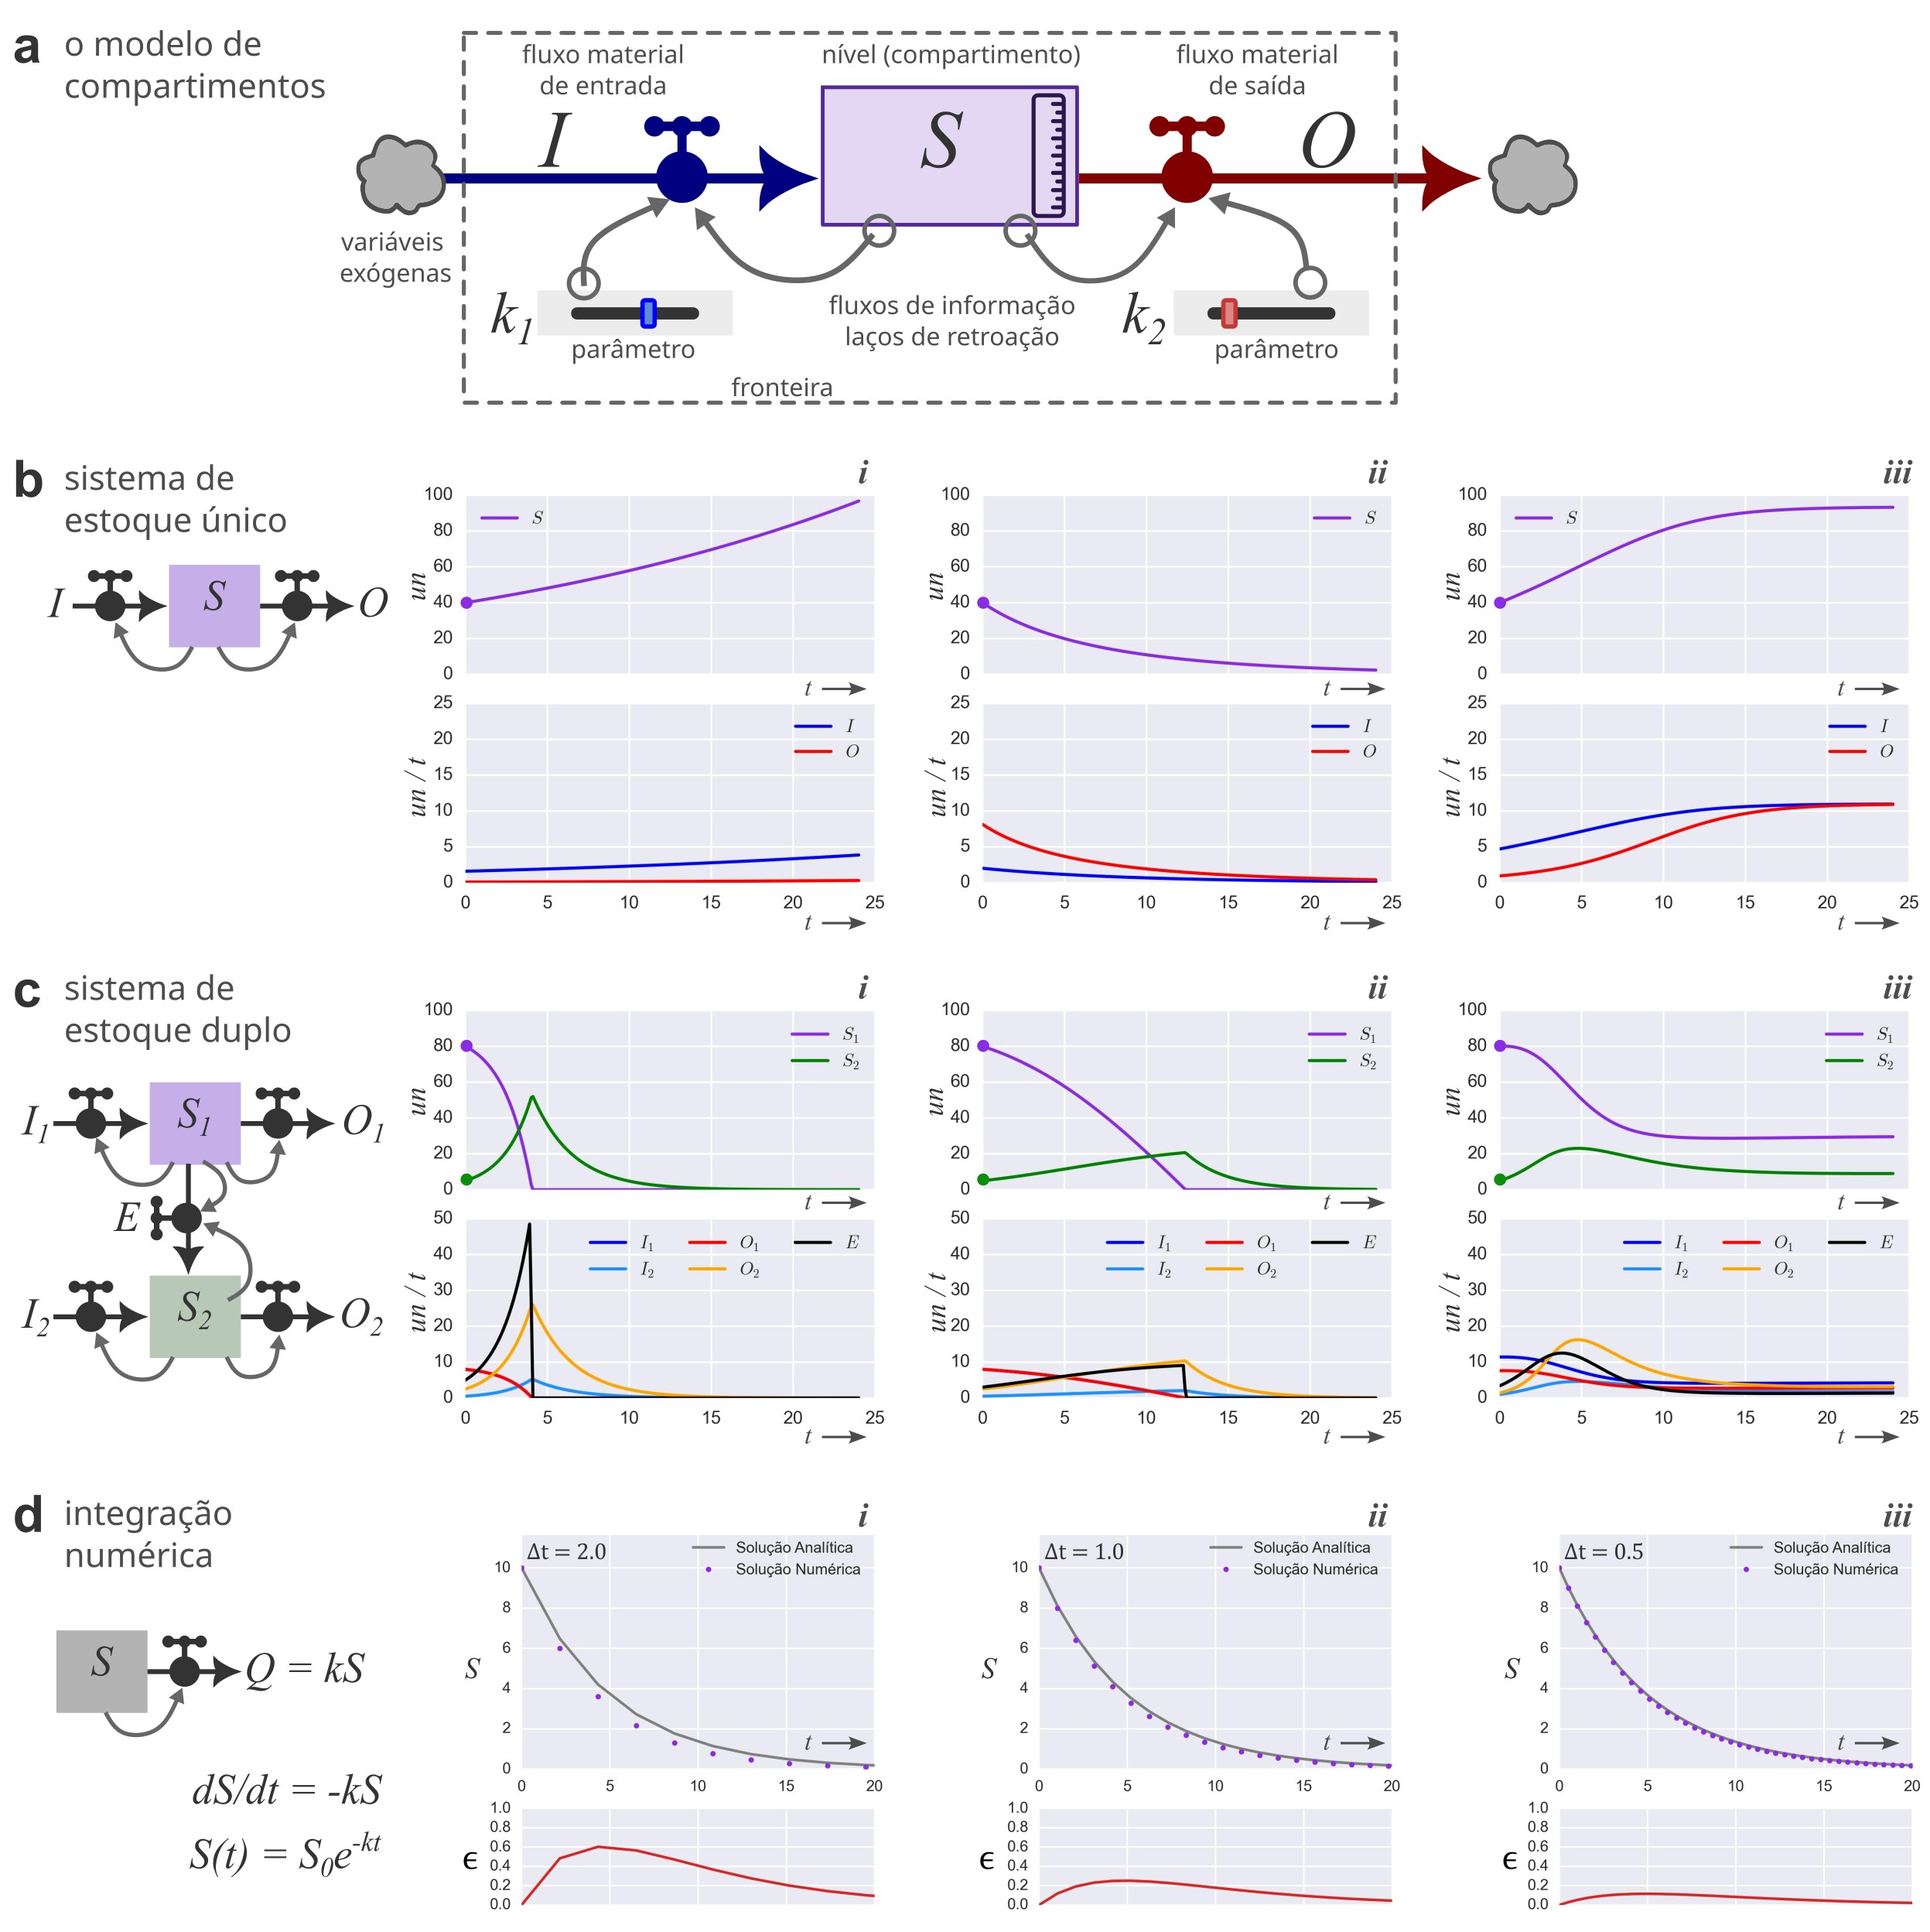
\includegraphics[width=0.95\linewidth]{figs/fig_dynamics.jpg}		
	\caption[Dinâmica de Sistemas e o modelo de compartimentos]
	{\textbf{---\;Dinâmica de Sistemas e o modelo de compartimentos.}\; O modelo de compartimentos consiste na arquitetura básica para se construir modelos no âmbito da Dinâmica de Sistemas. O sistema é resolvido numericamente, fazendo emergir padrões complexos.\;\textbf{a}\;---\;Diagrama de laços causais: o nível do compartimento $S$ muda a partir da atuação de fluxos materiais de entrada $I$ e de saída $O$. Fluxos de informação relacionam o nível com os fluxos materiais através da retroação, que é regulada por parâmetros do modelo (como $k_1$ e $k_2$). A \textbf{fronteira} do sistema não deve negligenciar grandes retroações com as variáveis exógenas.\;\textbf{b}\;---\;Simulações com o modelo de estoque único, com diferentes dominâncias entre os fluxos materiais de entrada e saída: crescimento exponencial (detalhe \textrm{\textit{i}}); decaimento exponencial (detalhe \textrm{\textit{ii}}), e; curva logística (detalhe \textrm{\textit{iii}}); \;\textbf{c}\;---\;Simulações com o modelo de estoque duplo, onde o nível $S_2$ esgota $S_1$ com um fluxo de extração $E$: sobrecarga e colapso rápido (detalhe \textrm{\textit{i}}); sobrecarga e colapso adiado (detalhe \textrm{\textit{ii}}), e; equilíbrio sustentável (detalhe \textrm{\textit{iii}}).\;\textbf{d}\;---\;A integração numérica introduz o erro de truncamento $\epsilon$, que pode ser minimizado com passos de tempo $\Delta t$ suficientemente curtos (detalhes \textrm{\textit{i}} a \textrm{\textit{iii}}). O comportamento geral do sistema não deve ser sensível ao passo de tempo $\Delta t$.
	}
\label{fig:sys:dynamics}  % use qualitative label			
\end{figure}

\par  Como já mencionado, entender a \textit{estrutura} de um sistema modelado é a chave para prever o seu \textit{comportamento}. Nesse rumo, o isomorfismo estrutural postulado por Bertalanffy torna-se, no âmbito da Dinâmica de Sistemas, o que Donella Meadows chama de \say{zoológico de sistemas}: um conjunto de sistemas que exibem \textit{comportamentos arquetípicos}, que podem ser generalizados para uma ampla gama de exemplos reais \cite{meadows2008}. Um bom ponto de partida nesse contexto é considerar o modelo mais simples possível, que é aquele que possui um único compartimento, governado pela Equação \eqref{eq:balance} (Figura \ref{fig:sys:dynamics}b). Ainda que simples, diferentes comportamentos se manifestam, a depender da \textit{dominância} de um fluxo sobre o outro. No caso da prevalência da entrada $I$ sobre as saída $O$, o nível $S$ do compartimento tenderá a aumentar (detalhe \textrm{\textit{i}} na Figura \ref{fig:sys:dynamics}b). Se existir retroação positiva, o padrão será de a \gls{curve-exp-grw}. No caso da prevalência do fluxo de saída, a tendência será de redução do nível $S$ (detalhe \textrm{\textit{ii}} na Figura \ref{fig:sys:dynamics}b). Aqui, a existência de retroação produz a \gls{curve-exp-dec}. Um exemplo concreto para esse sistema arquetípico é uma cultura de células (como bactérias ou fungos), crescendo em uma placa de Petri sem maiores limitações nutricionais. Quanto mais micro-organismos se reproduzem (fluxo de entrada), mais novas gerações são adicionadas na população total, que cresce exponencialmente. Mas, simultaneamente, o confinamento cada vez maior de células implica no acúmulo de resíduos tóxicos do seu próprio metabolismo, o que aumenta também a mortalidade (fluxo de saída). Esses dois fluxos atuam como um \gls{loop-rei} e um de \gls{loop-bal}, competindo pela dominância ao longo do tempo, produzindo padrões mais intricados do que simplesmente crescimento ou decaimento, como a \gls{curve-log} (detalhe \textrm{\textit{iii}} na Figura \ref{fig:sys:dynamics}b). 

\par Um segundo passo nessa linha é considerar os comportamentos que emergem a partir do \textit{acoplamento} de dois ou mais compartimentos. Meadows explora o modelo básico com dois compartimentos, em especial quando o nível $S_1$ do primeiro consiste em uma fonte de insumos $E$ para o nível $S_2$ do segundo (Figura \ref{fig:sys:dynamics}c). Esse é o caso, por exemplo, quando a cultura de células mencionada anteriormente possui recursos nutricionais limitados. Na verdade, esse arranjo é o arquétipo de qualquer sistema produtor-consumidor, o que inclui a própria economia global (recursos naturais e capital). Um padrão notável que emerge desse sistema é a \gls{curve-oac}, que ocorre quando o laço de equilíbrio no consumo dos recursos disponíveis não existe ou é muito fraco, fazendo o nível do segundo compartimento crescer rapidamente até esgotar a sua própria fonte, resultando finalmente em uma queda igualmente rápida (detalhe \textrm{\textit{i}} na Figura \ref{fig:sys:dynamics}c). A introdução de \textbf{retroações duplas} e \textbf{limiares de ativação} para atenuar ou mesmo suspender o consumo dos recursos podem tanto adiar o colaspo (detalhe \textrm{\textit{ii}} na Figura \ref{fig:sys:dynamics}c) quanto estabelecer um \textbf{equilíbrio sustentável} no longo prazo\footnote{No caso da economia global, esse cenário otimista é denominado de \textit{declínio próspero} por Odum e Odum \cite{odum2008}} (detalhe \textrm{\textit{iii}} na Figura \ref{fig:sys:dynamics}c). Além disso, a introdução de \textbf{atrasos} no fluxo de informações passam a produzir nos níveis, oscilações estáveis (amortecidas naturalmente) ou oscilações instáveis (amplificadas e caóticas). É fácil perceber que a complexidade e diversidade de comportamentos cresce vertiginosamente à medida que novos compartimentos e retroações são introduzidas nos modelos. A vantagem da Dinâmica de Sistemas, com sua natureza estritamente computacional, reside na capacidade de simular o sistema passo a passo a partir das relações básicas entre os compartimentos, eliminando a necessidade de se resolver explicitamente os sistemas de equações diferenciais não-lineares. Com isso, os padrões de crescimento, decaimento, saturação, colapso e oscilações simplesmente emergem.

\section{Um protótipo de modelo hidrológico} \label{sec:systems:model}

\par Com aquilo que foi apresentado até o momento, finalmente chegamos a uma posição adequada para introduzir um protótipo de modelo hidrológico. Nessa linha, o objetivo aqui é estabelecer as implicações básicas que a Dinâmica de Sistemas traz para a modelagem hidrológica por meio de um modelo exploratório e minimalista. Aprofundamentos teóricos e práticos, tanto sobre os processos hidrológicos quanto sobre modelos mais detalhados, serão articulados no próximo capítulo. 

\par Como salientado na Seção \ref{sec:sys:process}, todo processo de modelagem se inicia a partir de um \textit{modelo perceptual}. Assim, o modelo minimalista surge aqui de algumas percepções, em especial a de que uma bacia hidrográfica possui pelo menos duas formas diferentes de \textit{responder} aos eventos de chuva: uma mais rápida, a outra mais lenta. A \gls{hydro-response} rápida se manifesta nas enchentes dos rios que ocorrem após as chuvas. Já a resposta hidrológica lenta se evidencia durante o tempo seco, quando os rios continuam a escoar, mesmo após muitos dias ou mesmo meses sem chover. Nessa linha, assume-se que a resposta rápida está mais relacionada com processos superficiais, enquanto que a resposta lenta associa-se a processos subterrâneos. A primeira relação deriva da percepção de que bacias altamente impermeáveis ou com solos rasos produzem grandes enxurradas (resposta rápida). Por outro lado, as nascentes de riachos e áreas úmidas de fundos de vale em bacias mais preservadas reforçam a percepção do papel da água subterrânea em sustentar o escoamento de base dos rios durante o tempo seco. Um detalhe perceptual importante, que podemos já introduzir aqui, é que nem toda chuva produz uma resposta rápida, sendo necessário superar um certo \textit{nível de ativação}, como a interceptação da água no dossel ou o preenchimento das depressões do terreno que não são conectadas. Superado esse limiar, a \textit{saturação} incremental da superfície produz uma resposta rápida cada vez maior, que só irá cessar quando a superfície estiver novamente seca. Isso ocorre em razão do \textit{nível de conectividade} da superfície -- ou seja, é preciso mais água para conectar bolsões de água isolados com as saídas disponíveis (em canais ou macro-poros). Independentemente das formas de resposta, a água também precisa se deslocar por uma rede de canais até atingir a saída da bacia hidrográfica. Isso reforça outra percepção relevante, a de que o deslocamento da água implica em uma atenuação dos pulsos de resposta pelos efeitos de dissipação de energia. Por fim, uma última percepção refere-se ao fluxo de saída da \acrfull{et}. Nesse caso, espera-se que a transpiração das plantas pelo dossel seja o fluxo inicial, seguindo então da evaporação da água na superfície. 

\par Uma vez estabelecido um modelo perceptual, podemos avançar sobre um modelo conceitual a partir do enfoque da Dinâmica de Sistemas. O diagrama desse modelo é exibido na Figura \ref{fig:sys:proto}a. Assim, o primeiro passo para tanto consiste em definir a fronteira do sistema modelado. No caso de modelos hidrológicos típicos, busca-se representar uma bacia hidrográfica, que é uma extensão da superfície terrestre atravessada pelo ciclo hidrológico. A bacia hidrográfica, portanto, é um sistema aberto aos fluxos de água que entram por meio da precipitação atmosférica $P$ (chuva, neve e orvalho) e aos fluxos de saída, que podem ocorrer tanto pelo escoamento $Q$ quanto pela \acrlong{et}, denotada aqui por $E$. Assim, os fluxos $P$ e $E$ são mantidos como variáveis exógenas, obtidos a partir de \gls{input-data} e atuando de fora da fronteira do sistema-alvo. Admite-se, portanto, que o estado interno do sistema não exerce influência causal sobre o valor dessas variáveis\footnote{Essa suposição torna-se cada vez mais frágil à medida que a escala da bacia evolui de uma pequena área para grandes regiões ou continentes [>>:todo citar exemplos e referências].}. É claro que, sendo um fluxo de saída, a \acrlong{et} depende da água existente no sistema, mas o seu fluxo \textit{potencial} é determinado sem vínculos causais. O escoamento $Q$, ou vazão de saída, por outro lado, constitui-se de um fluxo calculado pelo próprio modelo a partir da aplicação das suas equações de fluxo. Modelos com essa característica são frequentemente chamados de modelos \say{chuva-vazão}, embora essa denominação esconda o fato de que muitos outros fluxos são calculados para se estimar a vazão de saída.

\par O segundo passo na construção de um modelo conceitual envolve a configuração dos reservatórios\footnote{No contexto de modelos hidrológicos, utilizarei o termo \textit{reservatório} como sinônimo de \textit{compartimento}.} do sistema em estudo. Para tal, é essencial mobilizar o conceito de resposta hidrológica providenciado pelo modelo perceptual. Visando manter o modelo em uma condição minimalista, definimos apenas dois reservatórios de resposta: um para a resposta rápida, $S_1$, e outro para a resposta lenta, $S_2$. Esses reservatórios são acoplados verticalmente, de forma que a água precisa passar pelo reservatório de resposta rápida (superior) antes de alcançar o de resposta lenta (inferior). Esse esquema busca representar o balanço hídrico no solo, sendo intuitivo relacionar a resposta rápida aos processos na superfície e a resposta lenta aos processos no solo e subsolo. Contudo, devido à simplificação do modelo, essa interpretação deve ser considerada com cautela: a representação em apenas dois reservatórios é, essencialmente, uma síntese de vários subprocessos que poderiam ser mais especificados em um modelo mais detalhado. Além dos reservatórios acoplados, um terceiro reservatório, $S_3$, coleta tanto os fluxos rápidos quanto os lentos, atuando como um filtro sobre o sinal de ambos. O propósito deste reservatório é modelar os efeitos de atenuação e armazenamento durante a propagação da vazão na rede de canais antes se atingir a saída da bacia hidrográfica. Assim como no caso do balanço hídrico no solo, este reservatório abrange vários subprocessos que, em um modelo mais complexo, poderiam ser explorados em detalhe. Considerando que a área da bacia hidrográfica é constante, é conveniente, embora não obrigatório, expressar os níveis dos reservatórios $S_i$ em \textit{mm} de coluna de água e os fluxos em \textit{mm}/$\Delta t$. Os reservatórios $S_1$ e $S_3$ (superfície e rede de canais, respectivamente) possuem capacidade total ilimitada, enquanto o reservatório $S_2$ (solo e subsolo) atinge sua capacidade máxima a partir de um certo nível, de forma que:
\begin{linenomath*}
\begin{equation}
\label{eq:max_capacity}
S_{2, t} \leq s_{2,\text{max}} \quad \forall ; i, t
\end{equation}
\end{linenomath*}
Em que $s_{2, \text{max}}$ é a \textit{capacidade máxima de armazenamento} de $S_2$, um parâmetro expresso em unidades de nível (\textit{mm}).

\par O terceiro passo, por fim, consiste em se definir as equações de fluxo que governam o balanço de água em cada reservatório. Nesse sentido, todos os três reservatórios funcionam como um \gls{linear-reserv}, o que implica que apresentam um fluxo de saída $Q_t$ diretamente proporcional ao nível $S_t$, ou seja:
\begin{linenomath*}
\begin{equation} 
	\label{eq:linear_reservoir}
	Q_{i, t} = \frac{1}{k_{i}} \cdot S_{i,t} \quad \forall \;  i, t 
\end{equation}
\end{linenomath*}
Em que $k_i$ é um parâmetro com unidades de tempo que é equivalente ao tempo de residência médio do reservatório $S_i$. Isso implica que quanto \textit{maior} o valor de $k_i$, mais \textit{lento} é o seu esvaziamento, como ilustrado na Figura \ref{fig:sys:proto}b (detalhes \textit{i} e \textit{ii}). Um reservatório linear é análogo a uma caixa de água com paredes verticais e um orifício poroso, que propicia um escoamento laminar diretamente proporcional à coluna de água. No caso do reservatório de resposta rápida $S_1$, o fluxo de saída $Q_1$ é o fluxo de transferência vertical da água para o reservatório $S_2$, sendo interpretável como a \textit{infiltração} da superfície para o interior do solo, com as devidas ressalvas de efetividade. Já no caso do reservatório $S_2$, o fluxo de saída $Q_2$ é a própria resposta lenta da bacia hidrográfica, interpretável como o \textit{escoamento de base} que o solo produz diretamente na rede de drenagem. Por fim, o fluxo de saída $Q_3$ é a \textit{vazão de saída} final, resultante da atenuação do escoamento pelo processo de propagação de vazão. O fluxo de saída rápida do reservatório $S_1$, denotado por $R$, apresenta uma formulação específica, que corresponde a uma hipótese de como que os processos rápidos, como o escoamento superficial, se desenvolvem na bacia hidrográfica. Assim como no fluxo de saída de um reservatório linear, $R$ é diretamente proporcional ao nível armazenado, com a diferença que o nível precisa superar um valor mínimo $s_a$ antes de começar a verter:
\begin{linenomath*}
\begin{equation} 
	\label{eq:fast_response}
 R_{t} = 
\begin{cases} 
    0 & \text{se } \quad S_{1,t} \leq s_a\\
    c \cdot (S_{1,t} - s_a) & \text{se } \quad S_{1,t} > s_a
\end{cases}
\end{equation}
\end{linenomath*}
Em que $s_a$ é o \textbf{nível de ativação} da resposta rápida, um parâmetro do modelo expresso em unidades de nível; e  $c$ é um \textit{coeficiente de escoamento}, com unidades de $t^{-1}$. Mas ao contrário do reservatório linear, o valor de $c$ não é constante, mas sim uma função do próprio nível $S_1$. Para os propósitos deste capítulo, vamos estabelecer simplesmente que a resposta rápida $R$ resulta de um \textit{processo de saturação} do reservatório $S_1$, de maneira que:
\begin{linenomath*}
\begin{equation} 
	\label{eq:fast_coeff}
	c = \frac{(S_{1,t} - s_a)}{(S_{1,t} - s_a) + s_c} \frac{1}{\Delta t} \quad \forall\;t
\end{equation}
\end{linenomath*}
Em que $s_c$ é o \textbf{nível de conectividade}, um parâmetro com as mesmas unidades do nível $S_1$ e que regula a velocidade do processo de saturação. O nível $s_c$ representa 50\% de conectividade, de forma que quanto maior o valor de $s_c$, mais lentamente ocorre a saturação do reservatório. À medida que o nível reservatório aumenta, o coeficiente de escoamento $c$ se aproxima assintoticamente de 1\footnote{A Equação \eqref{eq:fast_coeff} apresenta uma forma típica de processos de saturação encontrada em campos distintos, como, por exemplo, a \textbf{Equação de Michaelis-Menten} na cinética de reações químicas.}, como ilustrado na Figura \ref{fig:sys:proto}b (detalhes \textrm{\textit{iii}} e \textrm{\textit{iv}}). O termo $1/ \Delta t$ foi mantido na definição de $c$ para explicitar as suas unidades, ainda que ele seja efetivamente eliminado na equação de balanço (Equação \eqref{eq:balance_numeric}). Por substituição da Equação \eqref{eq:fast_coeff} na Equação \eqref{eq:fast_response}, chega-se na equação de fluxo para $R$ (no caso de $S_{1,t} > s_a$)\footnote{Um olhar cauteloso capta que a Equação \eqref{eq:fast_response_2} tem exatamente a mesma estrutura da fórmula empírica do método CN proposta pelo Soil Conservation Service para estimar o escoamento efetivo a partir de eventos de chuva e tipos de cobertura do solo. Este é um fato curioso que deve ser melhor estudado.}:
\begin{linenomath*}
\begin{equation} 
\label{eq:fast_response_2}
 R_{t} = \frac{(S_{1,t} - s_a)^2}{(S_{1,t} - s_a) + s_c} \quad \forall\;t
\end{equation}
\end{linenomath*}

\par Nesse modelo minimalista, o fluxo externo de \acrlong{et} $E$ atua no balanço hídrico do solo, sobre os reservatórios $S_1$ e $S_2$, de forma que $E = E_1 + E_2$. A drenagem da água, nesse caso, ocorre de baixo para cima, ou seja, o fluxo $E$ passa a atuar no reservatório superior $S_1$ apenas quanto o reservatório inferior $S_2$ estiver vazio. Ou seja, o fluxo de saída $E_2$ em $S_2$ corresponde à transpiração das plantas, que remove água no solo, e o fluxo de saída $E_1$ em $S_1$ corresponde à evaporação superficial. Assim, nota-se que os reservatórios $S_1$ e $S_2$ são \textit{deplecionados simultaneamente} por mais de um fluxo de saída. Para $S_1$, os fluxos de saída são $E_1$, $R$ e $Q_1$. Para $S_2$, os fluxos de saída são $E_2$ e $Q_2$. Esse é um bom ponto para se introduzir dois problema práticos em modelos de compartimentos na Dinâmica de Sistemas, que são o \gls{problem-congest-outputs} e o \gls{problem-simult-deplet}. O primeiro problema consiste na dificuldade de se determinar um dado fluxo de saída $O_{t,j}$ que \textit{também é uma entrada} em um compartimento com capacidade de armazenamento limitada. No caso do modelo hidrológico minimalista, isso ocorre no fluxo $Q_1$ (infiltração), que sai de $S_1$ (superfície) para $S_2$ (solo e subsolo). Mas como o reservatório $S_2$ é limitado por $s_{2, \text{max}}$ (Equação \eqref{eq:max_capacity}), existe uma retroação negativa de $S_2$ sobre $Q_1$, que pode ser interpretada pela noção de que o fluxo de infiltração é \textit{congestionável} pela umidade existente no solo. Afinal, se os poros do solo já estão ocupados com água, não importa o quanto existe de água disponível para infiltração armazenada na superfície. O \gls{flux-actual} $Q_{1,t}$, assim, é obtido ao se confrontar o \gls{flux-pot} de saída $Q^*_{1,t}$ com o \gls{flux-max} de entrada possível no próximo reservatório, que no caso de $S_2$ é definido pelo \gls{storage-deficit} $D_{2,t}$ dividido pelo passo de tempo $\Delta t$:
\begin{linenomath*}
\begin{equation} 
	\label{eq:congest_1}
 Q_{1,t} = 
\begin{cases} 
    Q^*_{1,t} & \text{se } \quad Q^*_{1,t} \leq D_{2,t} / \Delta t\\
    D_{2,t} / \Delta t & \text{se } \quad Q^*_{1,t} > D_{2,t} / \Delta t
\end{cases}
\end{equation}
\end{linenomath*}
Onde $D_{2,t}$ é calculado por:
\begin{linenomath*}
\begin{equation} 
	\label{eq:congest_2}
 D_{2,t} = s_{2, \text{max}} - S_{2,t}
\end{equation}
\end{linenomath*}
Essa solução pode ser generalizada para outros fluxos de saída congestionáveis\footnote{Nesse contexto, vale ressaltar que John Sterman defende que não se faça uso de estruturas condicionais do tipo \texttt{IF... THEN... ELSE} no código de simulação, sugerindo que uma alternativa para a Equação \eqref{eq:congest_1} do tipo $Q_{1,t} = \texttt{MIN}(Q^*_{1,t}, D_{2, t} / \Delta t)$ é mais robusta e legível \cite{sterman2000}. }. Quando um compartimento com capacidade limitada possui \textit{múltiplas} entradas simultâneas, então a solução precisa adotar uma abordagem análoga (mas inversa) ao outro problema mencionado, que é o problema da depleção simultânea. Esse problema, por sua vez, consiste na dificuldade de \textit{prevenir valores negativos} em um nível submetido a múltiplos fluxos de saídas e que é integrado numericamente pelo método de Euler. Em um sistema matematicamente contínuo, as diversas taxas de saída atuam suavemente sobre um dado nível $S_t$, de maneira que ele tende assintoticamente para zero. Mas o método de Euler, ao considerar que as taxas são constantes durante um intervalo discreto de tempo $\Delta t$, introduz o risco de que $S_{t+1}$ possa assumir valores negativos. A solução para esse problema é computar os fluxos de saída em três etapas. Na primeira delas se calcula o fluxo \textit{potencial} de saída total $O^*_t$ pela soma dos fluxos potenciais de saída individuais. Em termos mais genéricos, para $M$ fluxos potenciais de saída $O^*_{t,j}$:
\begin{linenomath*}
\begin{equation} 
\label{eq:simult_1}
 O^*_t = \sum_{j}^{M}O^*_{t, j} \quad \forall\;t
\end{equation}
\end{linenomath*}
A seguir, o fluxo \textit{real} de saída total $O_t$ é determinado ao se confrontar o fluxo potencial com o fluxo \textit{máximo} de saída possível que é o valor do próprio nível $S_t$ do reservatório dividido pelo passo de tempo $\Delta t$:
\begin{linenomath*}
\begin{equation} 
	\label{eq:simult_2}
 O_{t} = 
\begin{cases} 
    O^*_t & \text{se } \quad O^*_t \leq S_t / \Delta t\\
    S_t / \Delta t & \text{se } \quad O^*_t > S_t / \Delta t
\end{cases}
\end{equation}
\end{linenomath*}
A terceira etapa, enfim, consiste em calcular o valor dos fluxos reais de saída \textit{individuais}. Já que o método de Euler assume taxas de fluxo constantes, os fluxos reais de saída são diretamente proporcionais ao \textit{rateio} dos fluxos potenciais de saída:
\begin{linenomath*}
\begin{equation} 
	\label{eq:simult_3}
 O_{t, j} = \frac{O^*_{t, j}}{O^*_t} \cdot O_{t} \quad \forall\;t
\end{equation}
\end{linenomath*}

{\renewcommand{\arraystretch}{1.5}% for the vertical padding
\begin{table}[t!]
    \centering	
    \tiny
    \sffamily
    \rowcolors{2}{white}{rowgray}
    \begin{tabular}{ 
        >{\raggedright\arraybackslash}m{1cm}  
        >{\raggedright\arraybackslash}m{5cm}  
        >{\raggedright\arraybackslash}m{1cm}
        >{\raggedright\arraybackslash}m{1cm}
        >{\raggedright\arraybackslash}m{2cm}}
        \toprule
        \textbf{Componente} & \textbf{Nome} & \textbf{Dimensão} & \textbf{Unidade} & \textbf{Categoria} \\ 
        \midrule
        $S_1$ & reservatório de resposta rápida (superficial) & L & mm & nível \\ 
        $S_2$ & reservatório de resposta lenta (subterrâneo) & L & mm & nível \\ 
        $S_3$ & reservatório da rede de drenagem & L & mm & nível \\ 
        $P$ & precipitação & L/T & mm/h & fluxo (exógeno)\\
        $E$ & \acrlong{et} potencial & L/T & mm/h & fluxo (exógeno)\\ 
        $R$ & escoamento rápido ($S_1 \rightarrow S_3$) & L/T & mm/h & fluxo\\ 
        $Q_1$ & infiltração ($S_1 \rightarrow S_2$) & L/T & mm/h & fluxo\\ 
        $Q_2$ & escoamento lento ($S_2 \rightarrow S_3$) & L/T & mm/h & fluxo\\ 
        $Q_3$ & vazão de saída de $S_3$ & L/T & mm/h & fluxo\\ 
        $E_1$ & evaporação & L/T & mm/h & fluxo\\ 
        $E_2$ & transpiração & L/T & mm/h & fluxo\\ 
        $k_1$ & tempo de detenção de $S_1$ (superficial) & T & h & parâmetro \\ 
        $k_2$ & tempo de detenção $S_2$ (subterrâneo) & T & h & parâmetro \\ 
        $k_3$ & tempo de detenção $S_3$ (rede de drenagem) & T & h & parâmetro \\ 
        $s_a$ & nível de ativação da resposta rápida & L & mm & parâmetro \\ 
        $s_c$ & nível de conectividade de $S_1$ & L & mm & parâmetro \\ 
        $s_{2,\text{max}}$ & capacidade máxima de $S_2$ & L & mm & parâmetro \\ 
        \bottomrule
    \end{tabular}
    \caption[Resumo do protótipo de modelo hidrológico]{
    Resumo do protótipo do modelo hidrológico desenvolvido, listando as componentes de nível, fluxos e parâmetros. Pelo algo grau de agregação do do modelo, os nomes e significados das componentes devem ser interpretados com cautela, sendo na verdade processos efetivos que podem ser melhor detalhados e desagregados em versões mais complexas. 
    }
    \label{tbl:prototype}
\end{table} 
}

\par Tais problemas, inerentes à natureza computacional da Dinâmica de Sistemas, já indicam o próximo movimento no processo de modelagem: o desenvolvimento de um \textit{modelo procedural}, ou seja, um programa de computador. Na forma proposta acima, o modelo conceitual é simples o suficiente para ser implementado em uma \textit{planilha de cálculo}, em que as colunas representam as diferentes variáveis de armazenamento e fluxo e as linhas os passos de tempo da simulação. Para seguir o método de Euler, as fórmulas nas células de balanço dos reservatórios devem apontar para a linha anterior, nas colunas dos fluxos. Algumas colunas auxiliares devem ser criadas para implementar as etapas intermediárias dos fluxos potenciais e fluxos máximos. Além disso, certas células estáticas devem ser mantidas isoladas, como valor dos parâmetros $\Theta = \{k_1, k_2, k_3, s_a, s_c, s_{2, \text{max}}\}$, o valor das condições iniciais $\textbf{S}_{t=0} = \{S_{1, t=0}, S_{2, t=0}, S_{3, t=0}\}$ e o valor das variáveis exógenas $\Upsilon = \{P_t, E_t\}$. Uma alternativa mais robusta, no entanto, é implementar o modelo procedural a partir de um código, como \texttt{C}, \texttt{Fortran}, \texttt{Python}, etc. Uma estrutura simples de código deve ser baseado no paradigma funcional de computação, com três etapas acopláveis: 
\begin{enumerate}
    \item importação do dados de entrada;
    \item processamento do modelo, e;
    \item exportação dos dados de saída.
\end{enumerate}
Cada etapa possui suas características típicas e limitações técnicas, desde a definição do formato dos arquivos de dados ao uso de estruturas eficientes oferecidas pela linguagem de programação escolhida. Nesse rumo, um código apresenta duas vantagens fundamentais: uma cognitiva e outra operacional. A vantagem cognitiva é que um código explicita completamente as equações e próprio algoritmo computacional\footnote{Códigos altamente eficientes geralmente implicam em um sacrifício na legibilidade, o que reforça a importância de materiais suplementares como documentação e comentários.}. Planilhas de cálculo e demais interfaces gráficas, em contraste, acabam escondendo as fórmulas e a estrutura do algoritmo, tornando o modelo procedural um tanto inacessível em termos cognitivos. A vantagem operacional, por sua vez, é que um código permite o \textit{aninhamento} do processo de simulação em uma hierarquia maior de processos, como na execução de bateladas (múltiplas simulações em série ou paralelo) e no acoplamento com outros modelos (quanto o resultado de um é usado como dados de entrada em outro). Como veremos adiante, essa vantagem operacional é essencial para o diagnóstico e pesquisa de modelos.

% figure
\begin{figure}[t!] % place figure in the page
	\centering				
	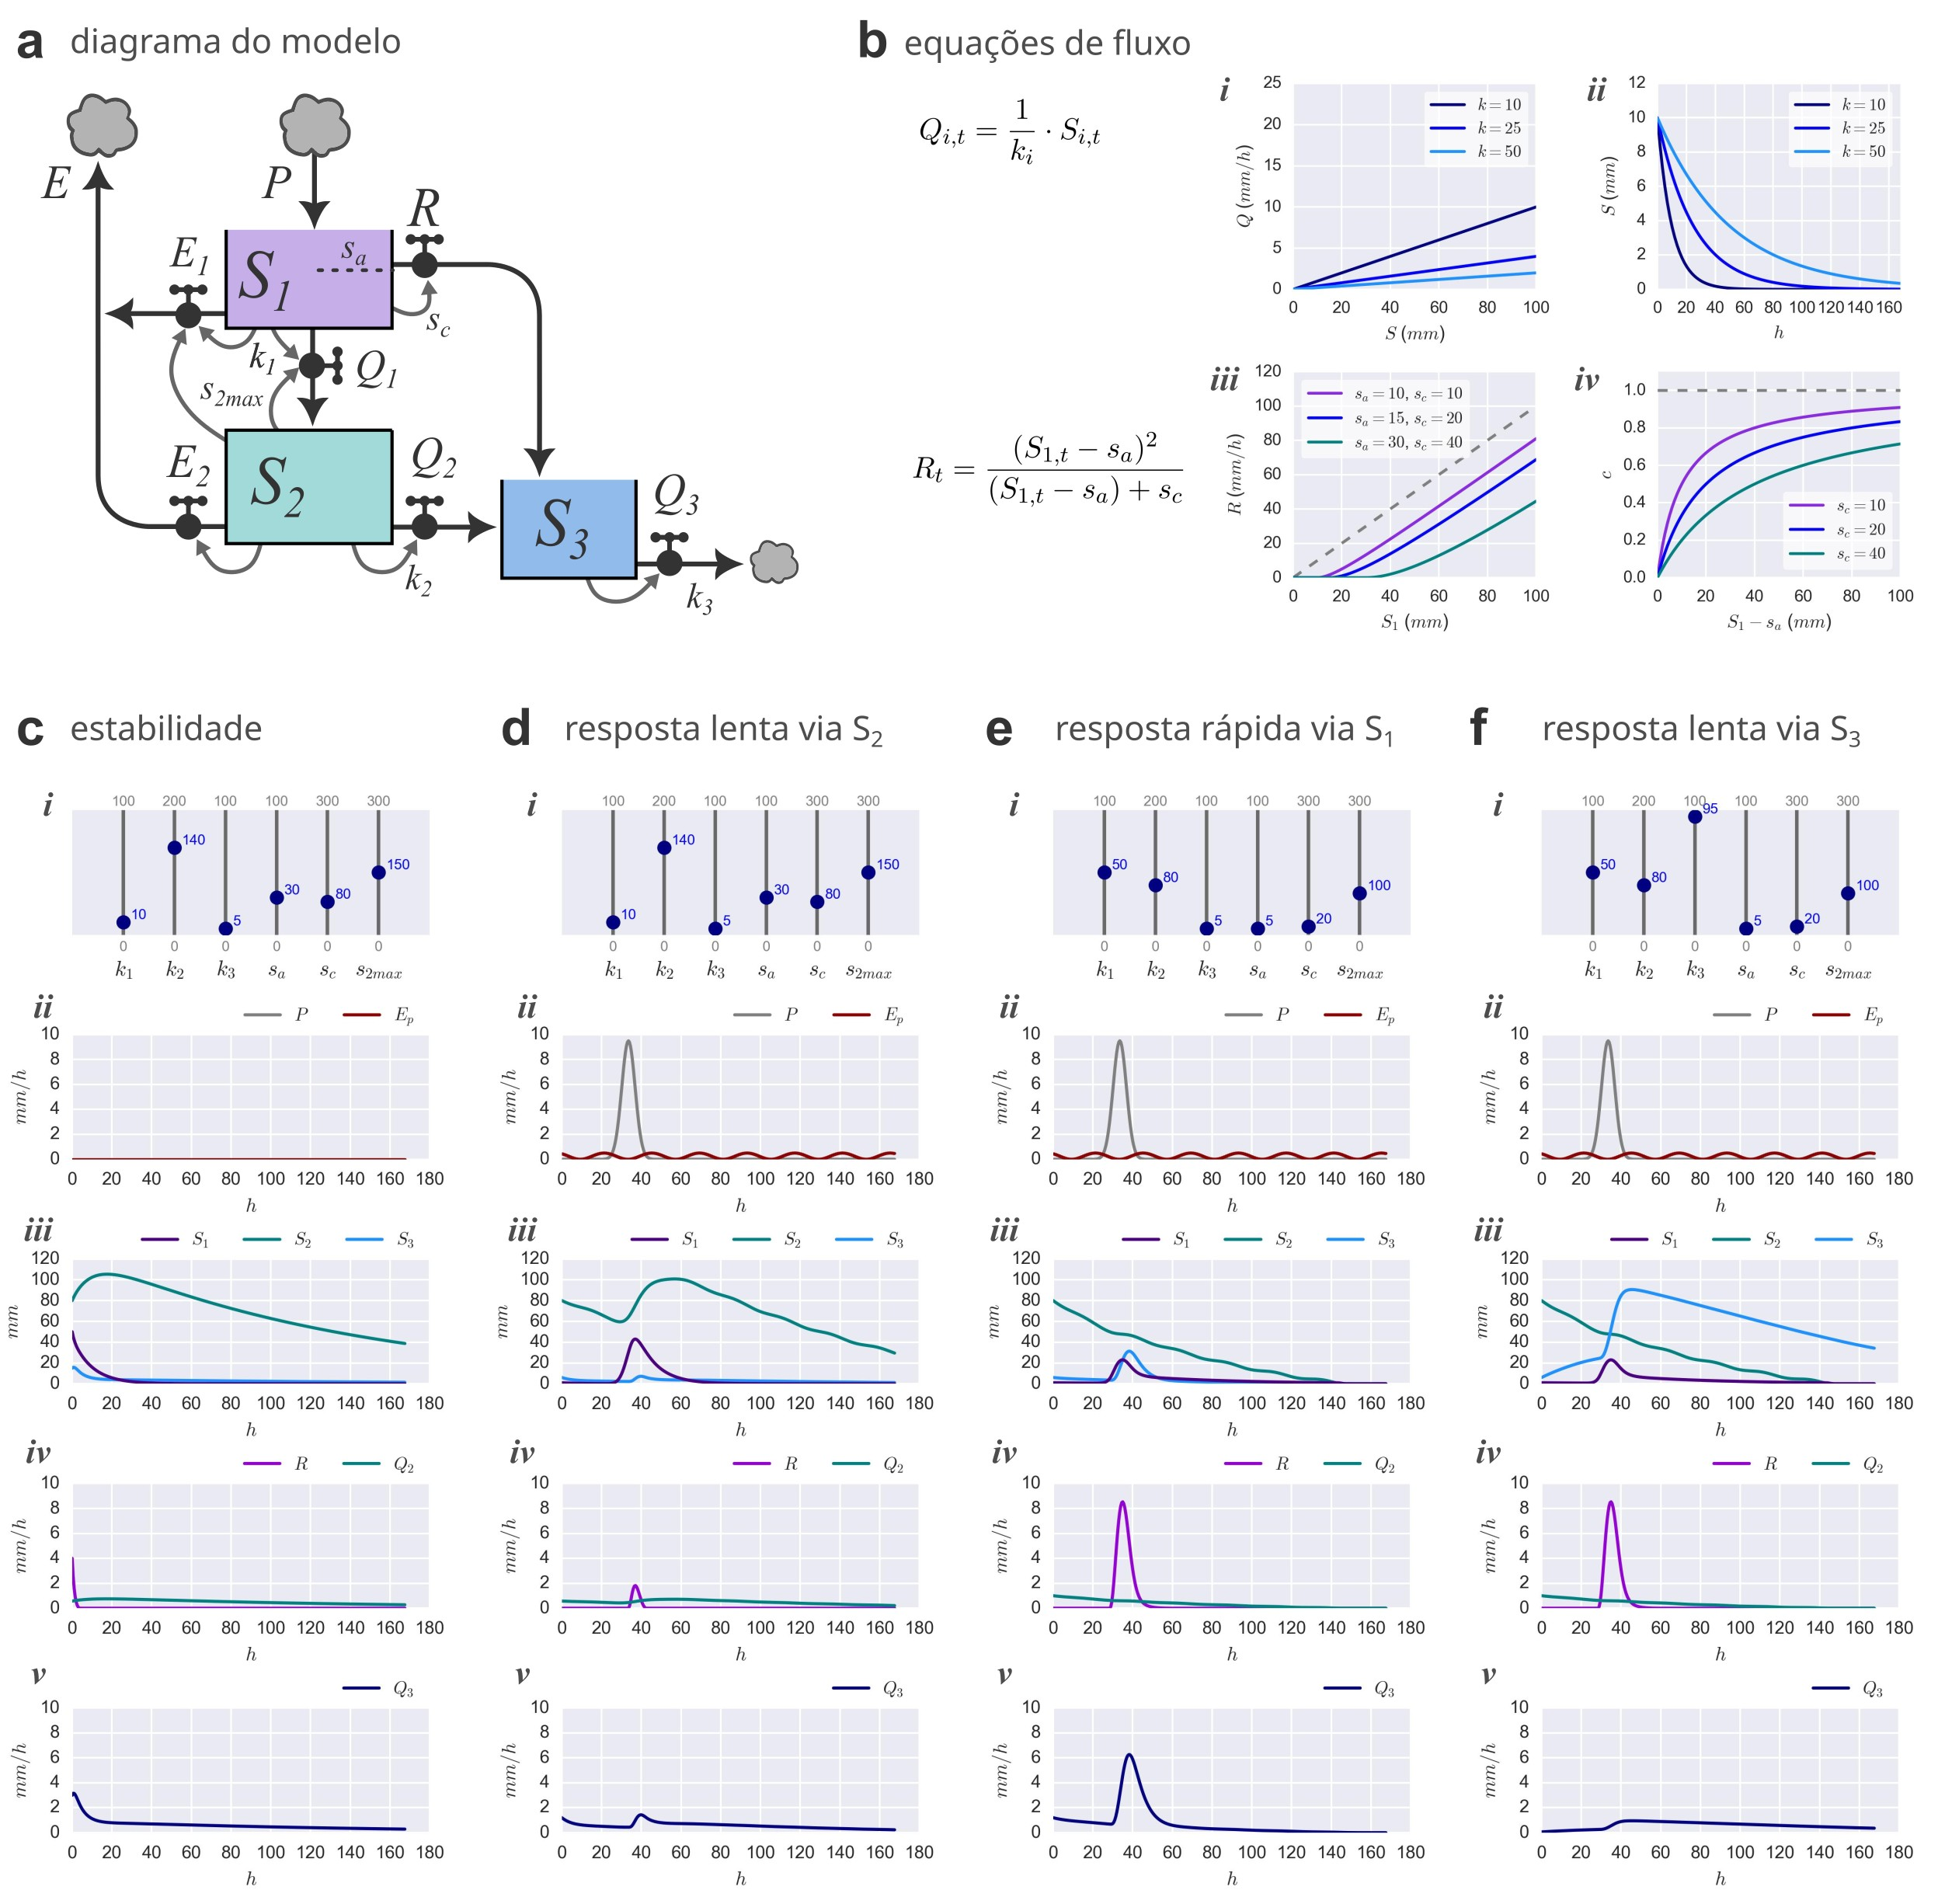
\includegraphics[width=0.95\linewidth]{figs/fig_minimodel.jpg}		
	\caption[Um protótipo de modelo hidrológico]
	{\textbf{---\;Um protótipo de modelo hidrológico e seu comportamento.}\;O modelo é mantido como minimalista para propósitos exploratórios.\;\textbf{a}\;---\;A estrutura do modelo é concebida com três reservatórios ($S_1$, $S_1$ e $S_3$) para representar mecanismos de resposta hidrológica lenta ou rápida. $S_1$ representa a superfície, $S_2$ representa o subsolo e $S_3$ representa a rede de drenagem. Com seis parâmetros que regulam os fluxos internos, o sistema é submetido aos fluxos exógenos de evapotranspiração $E$ e precipitação $P$. O reservatório $S_2$ é o único com capacidade limitada ($s_\text{2max}$).\;\textbf{b}\;---\;Duas equações regulam os fluxos (Equação \eqref{eq:linear_reservoir} e Equação \eqref{eq:fast_response_2}). A equação de decaimento exponencial para os reservatórios ($Q_i = S_i/k_i$, detalhe \textrm{\textit{i}}), em que o $k_i$ é o tempo de detenção. Quanto maior o valor de $k$, mais lentamente o reservatório se esvazia (detalhe \textrm{\textit{ii}}). A equação de resposta rápida ($R = c\cdot (S_1 - s_a)$, detalhe \textrm{\textit{i}}) é parecida, mas \textit{c} resulta de um processo de saturação da superfície ($c = (S_1 - s_a)/(S_1 - s_a + s_c)$, detalhe \textrm{\textit{ii}}). O processo é regulado pelo limiar de ativação $s_a$ e pelo nível de conectividade $s_c$.\;\textbf{c}\;---\;O sistema apresenta um comportamento estável -- se esvazia por conta própria, mesmo quando $P$ e $E$ são nulos (detalhe \textrm{\textit{ii}}). No caso, $S_2$ apresentou um pico à medida que a água de $S_1$ se infiltrava (detalhe \textrm{\textit{iii}}). Mas logo depois todos os reservatórios se esvaziaram.\;\textbf{d}\;---\;Uma configuração de parâmetros (detalhe \textrm{\textit{i}}) que define uma resposta lenta pela ação de $S_2$ (subsolo). No caso, um pulso de chuva $P$ com um máximo de 9.5 mm/h e uma oscilação diária de $E$ (detalhe \textrm{\textit{ii}}) resultam em uma vazão $Q_3$ atenuada (detalhe \textrm{\textit{iv}}); $R$ tem um máximo de apenas 2 mm/h, enquanto que o escoamento de base $Q_2$ sustenta a vazão durante a maior parte do período simulado (detalhe \textrm{\textit{iii}}).\;\textbf{e}\;---\;Uma configuração de parâmetros (detalhe \textrm{\textit{i}}) que define uma resposta rápida pela ação de $S_2$ (superfície). O mesmo pulso de $P$ e $E$ anterior resultam em um hidrograma típico de $Q_3$, com um máximo de 6 mm/h (detalhe \textrm{\textit{iv}}); $R$ exibe um máximo de 8 mm/h e o escoamento de base $Q_2$ é extinto em cerca de 140 horas (detalhe \textrm{\textit{iii}}).\;\textbf{f}\;---\;Uma configuração de parâmetros (detalhe \textrm{\textit{i}}) semelhante em (\textbf{e}), mas que define uma resposta lenta pela ação de $S_3$ (rede de drenagem). O mesmo pulso de $P$ e $E$ anterior resultam em uma vazão $Q_3$ atenuada (detalhe \textrm{\textit{iv}}) -- a sustentação da vazão é feita pelo amortecimento na rede de drenagem.
	}
\label{fig:sys:proto}  % use qualitative label			
\end{figure}

\par Antes de se realizar qualquer simulação computacional com o protótipo de modelo hidrológico desenvolvido, cabe aqui salientar alguns aspectos valiosos que a formalização do modelo perceptual em um modelo conceitual traz. Como já mencionado, a Dinâmica de Sistemas possui um espírito exploratório, que busca não apenas fazer predições confiáveis sobre um sistema-alvo, mas também usar os modelos para \textit{aprender} sobre o comportamento desse sistema, identificando com isso pontos de alavancagem úteis na tomada de decisão. Dito isso, consideremos por um momento que a teoria veiculada pelo modelo proposto é \textit{justificada}, o que nos liberta dos problemas apresentados no Capítulo 1. Se for o caso, o que podemos deduzir \textit{a priori} sobre o comportamento da bacia hidrográfica? Quais são seus pontos de alavancagem críticos quando se considera, por exemplo, o problema da segurança hídrica\footnote{Esse problema será explorado no Capítulo 4}?  

\par Diante dessas questões, o primeiro aspecto a se notar é que \textbf{o sistema é estável}, dominado por retroações que fazem os níveis dos reservatórios \textit{tenderem a zero}, como ilustrado pela simulação na Figura \ref{fig:sys:proto}c. Em outras palavras: os reservatórios $S_1$, $S_2$ e $S_3$ se esvaziam por conta própria\footnote{Em termos físicos: pela ação da gravidade.}, mesmo sem nenhuma ação externa (quando $P=0$ e $E=0$). Ao contrário de sistemas ecológicos, sociais e econômicos, não se espera do sistema proposto nenhuma forma de crescimento exponencial ou oscilações. Um segundo aspecto consiste em classificar o comportamento final do sistema em termos da sensibilidade ao fluxo de entrada $P$. Em um extremo, temos um comportamento de baixa sensibilidade, caracterizado pela dominância do mecanismo de resposta lenta em $S_2$ e alto tempo de residência em $S_3$. As simulações tanto na Figura \ref{fig:sys:proto}d quanto na Figura \ref{fig:sys:proto}f ilustram possibilidades desse comportamento. No outro extremo, temos um comportamento de alta sensibilidade, caracterizado pela dominância do mecanismo de resposta rápida em $S_1$ e baixo tempo de residência em $S_3$, como na simulação na Figura \ref{fig:sys:proto}e. Mantida a estrutura proposta e os mesmos fluxos exógenos $P$ e $E$, é claro que o comportamento dependerá estritamente do conjunto de parâmetros $\Theta = \{k_1, k_2, k_3, s_a, s_c, s_{2, \text{max}}\}$, ainda que diferentes valores possam eventualmente resultar em comportamentos similares (de alta ou baixa sensibilidade). Por exemplo, é possível reduzir a sensibilidade do sistema ao se aumentar tanto o limiar de ativação da resposta rápida ($ \uparrow s_a$) quanto o tempo de residência na rede de drenagem ($ \uparrow k_3$), ou dois, simultaneamente\footnote{Essa ambiguidade está diretamente associada ao problema da equifinalidade. Como apresentado no Capítulo 1, o maior número de evidências empíricas possíveis devem ser empregadas a para \textit{condicionar} o comportamento do modelo.}. Isso nos conduz para o terceiro e último aspecto, que são os pontos de alavancagem do sistema diante de problemas práticos, como a segurança hídrica. Para os propósitos desse capítulo, o problema da segurança hídrica define-se na dificuldade em \textit{garantir a disponibilidade de água em quantidade e qualidade adequados} para as atividades humanas. Portanto, se conclui que qualquer estratégia de alavancagem no sistema deve direcionar o sistema para reduzir a sua sensibilidade diante do fluxo de entrada, buscando um \gls{regular-effect}. No balanço hídrico do solo, isso se traduz em reduzir a dominância do mecanismo de resposta rápida: aumentar o limiar de ativação, reduzir a conectividade superficial e reduzir o tempo de residência superficial. No caso da rede de drenagem, a única alternativa disponível é aumentar o tempo de residência com bacias de detenção, açudes ou mesmo barragens. 

\par Os aspectos levantados acima ilustram que a simples lógica dedutiva aplicada ao modelo conceitual desenvolvido possibilita identificar importantes \textit{insights} sobre o comportamento e sobre os pontos de alavancagem no sistema. Além disso, se o modelo traduz a essência do sistema-alvo, espera-se que versões mais detalhadas não eliminem a essência das conclusões obtidas, mas que introduza as nuances necessárias no processo de tomada de decisão baseado em modelos hidrológicos, a depender do problema necessário. Heterogeneidades na litologia, na pedologia, na cobertura do solo e na topografia certamente devem ampliar o leque de entendimentos teóricos e recomendações práticas. Apesar do salto observado entre o modelo perceptual (modelo mental) e o modelo conceitual, é claro que todo esse raciocínio pode esconder surpresas a partir de pontos cegos e interações não intuitivas entre as partes do sistema. Ademais, a suposição de que a teoria veiculada é justificada foi um movimento provisório: é preciso testar o modelo diante de evidências empíricas. Assim, a única saída para se fazer afirmações mais firmes é simular o modelo com técnicas de diagnóstico, que são apresentadas a seguir.

\section{Diagnóstico} \label{sec:sys:diags}

\par O \gls{model-diags} consiste em um vasto conjunto de técnicas aplicadas para se avaliar a \textit{adequação} de um modelo. Antes da justificação empírica, que é um teste crucial, um modelo precisa ser adequado pelo ângulo conceitual, técnico, prático e comportamental. Afinal, um modelo estatístico extremamente adequado em termos empíricos pode ser diretamente obtido com técnicas de otimização, como aprendizado de máquina. Mas o quê se pode \textit{aprender} sobre o sistema-alvo com um modelo estatístico? Um modelo estatístico sobre-ajustado aos dados disponíveis, por exemplo, pode ser útil para \textit{interpolações}, mas não para \textit{extrapolações}. Um modelo desse tipo não contribui muito no entendimento de como o sistema \textit{se comportaria} diante de uma dada política de alavancagem ou um cenário de futuro que jamais foi observado. A busca por aprendizado, no âmbito da Dinâmica de Sistemas, implica que a modelagem é um processo de inferência \textit{dedutiva}, que requer uma definição robusta e confiável das sentenças antecedentes (hipótese principal e auxiliares) antes da produção das suas sentenças consequentes (resultados simulados). Nesse rumo, John Sterman sugere uma lista de doze estratégias gerais para diagnosticar essas adequações, exibidas na Tabela \ref{tbl:tests}, aprimorando as propostas iniciais de Jay Forrester \cite{sterman2000}. Originalmente, ele utiliza a expressão \say{teste de modelos}, mas aqui o termo \say{teste} será reservado para quando se define explicitamente um \textit{critério de rejeição}. 

{\renewcommand{\arraystretch}{1.5}% for the vertical padding
\begin{table}[t!]
     % placed  here
    \centering	
    \tiny
    \sffamily
    \rowcolors{2}{white}{rowgray}
    \begin{tabular}{ 
 >{\raggedright\arraybackslash}m{2.75cm}  
 >{\raggedright\arraybackslash}m{5cm}  
 >{\raggedright\arraybackslash}m{5cm}}
        \toprule
        \textbf{Diagnóstico}$^*$& \textbf{Propósito}& \textbf{Procedimentos}\\ 
        \midrule
        \textbf{1. Adequação da fronteira} & Diagnosticar se as variáveis exógenas do modelo não implicam em negligências causais graves.& Explicitar o sistema e suas variáveis endógenas e exógenas em diagramas de laços causais.\\         
        
        \textbf{2. Adequação da estrutura} & Diagnosticar se a estrutura (incluindo equações de fluxo) estão de acordo com o modelo perceptual e não violam princípios teóricos básicos. O grau de agregação também precisa ser útil em termos práticos.& 
        Inspecionar equações e diagramas causais; explicitar as perguntas de tomada de decisão relacionas com os resultados esperados.\\        
        
        \textbf{3. Consistência dimensional} & Diagnosticar se as equações e parâmetros são consistentes e fazem sentido com relação a fenômenos reais.& 
        Inspecionar equações; Análise dimensional; Racionalizar sobre a teoria subjacente.\\ 
        
        \textbf{4. Distribuição dos parâmetros} & Diagnosticar o quanto distribuições dos valores estão de acordo com expectativas conceituais e empíricas.& Obter distribuições anteriores a partir de opinião especialista.\\        
        
        \textbf{5. Estudos comparativos (famílias de sistemas)} & Diagnosticar se a distribuição de parâmetros é consistente diante de sistemas-alvo da mesma família. Ex: diferentes bacias hidrográficas;& Obter distribuições de parâmetros condizentes com o maior número de membros possíveis de sistemas (modelo generalista).\\        
        
        \textbf{6. Erro de integração} & Diagnosticar se os resultados não são sensíveis ao intervalo de tempo e ao método de integração numérica.& Reduzir o passo de tempo; mudar o método de integração numérica.\\        
        
        \textbf{7. Condições extremas} & Diagnosticar o quanto o modelo procedural é robusto diante de valores muito altos ou muito baixos.& Simular o modelo em condições sintéticas com choques extremos nos valores.\\

        \textbf{8. Análise de sensibilidade} & Diagnosticar como variações nos parâmetros do modelo afetam os resultados, identificando parâmetros críticos para o comportamento do sistema. & Aplicação de técnicas exploratórias, como o Método de Monte Carlo, para amostragens aleatórias no espaço dos parâmetros. Uso de técnicas de busca para identificar cenários críticos e revelar políticas de alavancagem inusitadas.\\
        
        \textbf{9. Comportamento anômalo} & Diagnosticar comportamentos inesperados do modelo que possam indicar erros na formulação ou \textit{insights} importantes sobre o sistema modelado. & Submissão do modelo ao teste de encapsulamento; descartar.\\
        
        \textbf{10. Adequação empírica} & Diagnosticar se o modelo é capaz de reproduzir comportamentos observados no sistema-alvo, ajustando parâmetros para melhorar a aderência com os dados empíricos. & Comparação das saídas do modelo com dados observados, utilizando métricas como MAE, RMSE, e coeficientes como o de determinação e KGE.\\
        
        \textbf{11. Comportamento surpreendente} & Diagnosticar se os resultados de modelagem supreendem o público-alvo em alguma medida,  revisando seus modelos mentais.& 
        Comunicação eficaz dos resultados; revelar nuances e detalhes; demonstrar mecanismos não-intuitivos.\\  
        
        \textbf{12. Impactos positivos práticos} & Diagnosticar se a modelagem trouxe impactos positivos práticos no processo de tomada de decisão.& Preparar indicadores de impactos do modelo; documentação técnica; reprodutibilidade.\\  
        \bottomrule
    \end{tabular}
    \caption[Diagnóstico de modelos.]{
    \textbf{Diagnóstico de modelos no âmbito da Dinâmica de Sistemas.}\; --- \;Resumo dos doze \say{Testes de modelos}  propostos por John Sterman, dando sequência aos testes propostos por Jay Forrester. Adaptado de Sterman \cite{sterman2000}.
    }
    \label{tbl:tests}
\end{table}
}

\par Entre os diagnósticos conceituais, é essencial se avaliar a \textbf{adequação da fronteira}. Como ilustrado no protótipo de modelo hidrológico, uma premissa importante é que o armazenamento e os fluxos de água na bacia hidrográfica (as variáveis endógenas) não exercem influência sobre a precipitação e a evapotranspiração potencial (as variáveis exógenas). Essa suposição talvez seja questionável para grandes bacias hidrográficas, quando a evapotranspiração em uma região se converte em precipitação, seja localmente (núcleo de condensação de nuvens [>>:cite]) ou em outras partes (efeito de rios voadores [>>:cite]). Assim, à medida que se muda de uma escala local para uma escala continental, negligenciar as interações causais do sistema meteorológico e climático com os processos hidrológicos terrestres tende a ser cada vez mais inadequado. Outra avaliação conceitual básica é a \textbf{adequação da estrutura} do modelo, tanto em termos teóricos (princípios físicos) quanto em termos práticos (tomada de decisão). A estrutura do modelo deve garantir que não sejam violados princípios físicos, tais como a conservação de massa, a não-negatividade dos níveis e determinados processos irreversíveis. Para exemplificar, Sterman descreve um modelo econômico que apresentava resultados notáveis ao simular o mercado de couro, mas isso acontecia porque o modelo revertia o couro produzido \textit{de volta} em vacas assim que fosse necessário \cite{sterman2000}. Da mesma forma, é importante avaliar se o nível de agregação do modelo atende às necessidades pré-estabelecidas do processo decisório. Em modelagem hidrológica, o protótipo mencionado acima dificilmente seria útil para identificar áreas prioritárias de ação numa bacia hidrográfica, devido à sua natureza altamente agregada. 

\par Outros dois diagnósticos conceituais relacionados envolvem a \textbf{consistência dimensional} e a \textbf{distribuição dos parâmetros}. Essa avaliação relaciona-se com o \textit{significado} dos parâmetros nas equações de fluxos e a distribuição dos seus valores. Quando se parte de uma lógica dedutiva, as equações de fluxo precisam fazer sentido teórico (afinal, \textit{elas veiculam uma teoria}) e seus parâmetros devem apresentar nomes e unidades consistentes que sejam equivalentes (ao menos em termos efetivos) com processos reais. Para Sterman, parâmetros e variáveis com nomes e unidades que não fazem sentido no mundo real são \textit{sintomas de que a teoria sobre o sistema-alvo está mal formulada}. Além disso, os valores dos parâmetros em si também precisam atender expectativas conceituais. Como diferentes combinações de parâmetros podem resultar em comportamentos finais similares (problema da equifinalidade), certas combinações de parâmetros podem até ser empiricamente adequadas, mas teoricamente duvidosas. Por exemplo, em uma bacia hidrográfica montanhosa sem reservatórios artificiais, espera-se uma baixa atenuação do pulso de vazão na rede de drenagem, ou ao menos menor que em bacias mais planas, com planícies de inundação. Assim, \textbf{estudos comparativos} entre sistemas distintos, mas da mesma \textit{família}, e a definição de distribuições anteriores pela \textbf{opinião de especialistas} ajudam a descartar valores de parâmetros inconsistentes\footnote{Espera-se que a opinião especialista \textit{informe} sobre a distribuição anterior de parâmetros com evidências empíricas qualitativas de seus modelos perceptuais que não foram transformadas em dados quantitativos. Ainda assim, é preciso ter cautela para não transformar esse processo em um \textbf{viés de confirmação}, mantendo uma abertura para que as anomalias empíricas possam atuar para refutar as teorias postuladas pelos modelos. Uma saída para isso é manter as probabilidades posteriores dentro de um limiar mínimo.}. 

\par Do lado técnico, um diagnóstico crucial é o \textbf{teste de integração numérica}, que foi descrito na Seção \ref{sec:sys:dynamics}. Cumpre ressaltar que \textit{nenhuma simulação é informativa se o seu resultado decorre de instabilidades numéricas}. Assim, esse teste consiste em avaliar se o comportamento do sistema segue o princípio da insensibilidade temporal. Outro diagnóstico nessa linha consiste em submeter o modelo sob \textbf{condições extremas e limítrofes}, como valores muito altos de fluxos de entrada e de saída. Essa é uma avaliação da robustez técnica, pois são nessas condições não-usuais (mas possíveis) que problemas no modelo procedural podem surgir, como erros na representação numérica das estruturas de dados (\textit{overflow} e \textit{underflow}) e violações da não-negatividade nos níveis simulados. Por exemplo, uma variável de nível discreta (como uma população) pode ser instanciada por uma estrutura de dados de número positivo, inteiro e 16 bits -- o que traz ganhos de memória interessantes, ao contrário de 64 bits em ponto flutuante. Mas essa estrutura de dados possui um limite numérico superior de 65535 -- valores acima disso retornam para números baixos, um erro de \textit{overflow} que pode tornar os resultados das simulações desprovidos de qualquer sentido. Nesse caso, é preciso se certificar que um código mais eficiente não compromete a robustez das simulações diante de condições extremas mas que são factíveis.

\par O diagnósticos que avaliam o comportamento do modelo incluem a \gls{sal}, a \textbf{detecção de anomalias} e a \textbf{adequação empírica}. Essas avaliações formam um espectro em termos da justificação. De um lado, a análise de sensibilidade busca entender como o sistema responde diante de mudanças nos seus elementos, tais como fluxos de entrada e valores de parâmetros. Nesse caso, a abordagem é exploratória, sem comprometimentos maiores com a justificação. Do outro lado, a adequação empírica busca encontrar os conjuntos de parâmetros que condicionam o sistema modelado a reproduzir o comportamento observado. Evidentemente, esse é o único teste capaz de apontar a necessidade de revisões importantes no processo de modelagem, pois é nele que a teoria é diretamente confrontada com as evidências disponíveis. Ainda assim, a rejeição do modelo proposto só é possível a partir do paradigma de modelagem discutido na Seção \ref{sec:epis:under} (Capítulo 1), que aplica um teste de encapsulamento de um conjunto de modelos empiricamente adequados. Uma abordagem puramente confirmatória, em contraste, busca \say{calibrar} os parâmetros do modelo de maneira a se identificar um único conjunto de parâmetros tido como adequado.

\par De uma forma ou de outra, os diagnósticos de comportamento em geral demandam que se realize uma ampla avaliação do \gls{space-params} $\Omega_{\Theta}$, o espaço matemático com $N$ dimensões criado pelos $N$ parâmetros instanciados no modelo conceitual. Aqui, surge um entrave técnico, que é o \gls{problem-dimens}: a dificuldade de se avaliar detalhadamente o espaço paramétrico $\Omega_{\Theta}$ em um tempo razoável de simulação. Por exemplo, considere uma \gls{brute-force}\footnote{Também denominado método da enumeração ou método da força-bruta.} em $M$ intervalos regulares na faixa estimada para cada parâmetro $\Theta_i$, com $i \in \{1, ..., N\}$. Segue disso que o número de simulações $n_s$ em uma amostragem exaustiva é $n_s = M^N$. Esse número pode assumir valores exorbitantes rapidamente: com $M=100$, seria preciso simular o modelo hidrológico proposto acima ($N=6$) um trilhão de vezes, $100^6 = 1.000.000.000.000$. Com um tempo de simulação de um segundo, essa avaliação iria levar em torno de \textit{31 mil anos} para ser concluída. Um tempo de simulação de um milésimo de segundo demandaria 31 anos. Para ser prática, a exploração no espaço paramétrico $\Omega_{\Theta}$ deve durar no máximo alguns dias, de preferência algumas horas ou minutos. 

\par Computadores mais potentes ajudam muito em contornar o problema da dimensionalidade, mas na prática a estratégia de amostragem também lança mão de métodos mais eficientes do que a amostragem exaustiva, que podem ser divididos em \textbf{técnicas exploratórias} e \textbf{técnicas de busca}, ainda que elas sejam em boa parte relacionadas. As técnicas exploratórias são variações do Método de Monte Carlo, mencionado na Seção \ref{sec:epis:bayes}, que fazem amostragens aleatórias sobre a faixa de valores esperados para os parâmetros $\Theta$. O objetivo aqui é apenas revelar as regiões do espaço paramétrico. Se uma distribuição de probabilidade anterior para os parâmetros está disponível (a partir de opinião especialista, por exemplo), essa amostragem pode ser \textit{ponderada pela densidade} da distribuição, fato que direciona a exploração mais em certas regiões do que em outras. Uma variação eficiente do Método de Monte Carlo consiste na amostragem aleatória \textit{sem reposição}, conhecida por \gls{lhs}, que garante uma distribuição mais espaçada dos conjuntos de parâmetros amostrados, evitando-se o risco de amostras redundantes. As técnicas de busca, por sua vez, consistem em técnicas de otimização que objetivam identificar regiões do espaço paramétrico que atendam especificações pré-definidas em termos do comportamento do sistema. No jargão da Pesquisa Operacional, essas técnicas maximizam ou minimizam uma dada \gls{obj-func}. Para tanto, uma ampla variedade de algoritmos de otimização podem ser implementados, como programação linear, programação dinâmica, escalada de gradiente, algoritmos evolucionários, cadeias de Markov, etc. O critério para escolha, no entanto, é condicional a diversas questões técnicas, em especial em modelos não lineares que exibem funções objetivos com múltiplos ótimos locais.

\par Na análise de sensibilidade, técnicas de exploratórias são aplicadas em se quantificar a sensibilidade numérica de cada parâmetro. Essa análise pode ser tanto \textit{local}, realizada ao se variar um parâmetro e manter o resto constante, quando \textit{global}, realizada por uma exploração mais completa do espaço paramétrico $\Omega_{\Theta}$ \cite{Saltelli2006}. Andrea Saltelli e colegas reforçam a importância da última, demonstrando que apenas a análise global tem o potencial de capturar interações e sinergias que emergem quando um dado conjunto de parâmetros muda ao mesmo tempo \cite{Saltelli2019}.  Mas também a análise de sensibilidade aplica técnicas de busca em explorações projetadas para se \textbf{descobrir cenários críticos} e revelar políticas de alavancagem inusitadas. Para ilustrar essa abordagem, John Miller aplicou duas técnicas de otimização (algoritmos genéticos e escalada de gradiente) sobre o modelo \texttt{Wolrd3} utilizado por Donella Meadows e colegas em \textit{Limites do crescimento}, de maneira a se descobrir cenários alternativos para a população mundial até 2100 \cite{miller1998}. Os resultados obtidos pelas buscas indicaram que é possível maximizar a população mundial em até seis vezes o previsto pelo cenário de base de Meadows (4 bilhões, com pico de 9 bilhões em 2050), mas também é possível minimizar a população até a metade do previsto. Esses diferentes modos de comportamento do mesmo sistema ajudam a entender melhor os parâmetros e fluxos críticos para a elaboração de políticas. Por exemplo, talvez seja desejável uma população mundial de 2 bilhões em 2100, mas não por causa de guerras, poluição e fome, e sim por causa de mudanças econômicas, tecnológicas e culturais que melhorem a qualidade de vidas das pessoas. 

\par Pelo lado da adequação empírica e detecção de anomalias, as técnicas exploratórias estão relacionados com a análise da incerteza dos parâmetros. Um método de especial relevância proposto na modelagem hidrológica é método \acrfull{glue}, proposto por Keith Beven e Andrew Binley, que aplica o Teorema de Bayes (Equação \eqref{eq:bayes-model-multi}) com uma função de verossimilhança informal $\mathcal{L}(E|H)$ \cite{beven1992}. Assim, a distribuição posterior dos parâmetros é obtida ao se condicionar a distribuição anterior com o histograma normalizado da verossimilhança $\mathcal{L}(E|H)$. Esse histograma, por sua vez, é calculado a partir de uma exploração robusta no espaço paramétrico $\Omega_{\Theta}$. As técnicas de busca, por outro lado, atuam no sentido de \say{calibrar} o modelo ao se maximizar a verossimilhança $\mathcal{L}(E|H)$, obtendo-se um único conjunto de parâmetros tido como adequado empiricamente\footnote{Em abordagens multi-objetivo, o conjunto de parâmetros considerado adequado empiricamente correspondem a uma fronteira de Pareto.}. De qualquer maneira, quando se tratando de modelos na Dinâmica de Sistemas, a verossimilhança informal $\mathcal{L}(E|H)$ geralmente é igualada a alguma estatística ponto-a-ponto, ou métrica de ajuste, que busca mensurar a aderência das variáveis simuladas aos dados observados. Com isso, quanto mais um ponto simulado $y_{M, i}$ se aproximar do seu ponto observado $y_{O, i}$ correspondente, maior é a sua adequação empírica. Uma métrica de ajuste típica é a média do erro absoluto \texttt{MAE}:
\begin{linenomath*}
\begin{equation} 
	\label{eq:mae}
 \text{MAE} = \frac{1}{n}\sum_{i}^{N} |y_{M, i} - y_{O, i}| 
\end{equation}
\end{linenomath*}
Uma alternativa que penaliza desproporcionalmente mais os erros maiores e menos os erros menores é a raiz quadrada da média do erro ao quadrado \texttt{RMSE}:
\begin{linenomath*}
\begin{equation} 
	\label{eq:rmse}
 \text{RMSE} = \sqrt{\frac{1}{n}\sum_{i}^{N} (y_{M, i} - y_{O, i})^2}  
\end{equation}
\end{linenomath*}
Tanto a métrica \texttt{MAE} quanto a métrica \texttt{RMSE} são positivas e apresentam as mesmas unidades da variável avaliada $y$, fato que faz delas difíceis de serem comparadas com outros modelos ou mesmo outras variáveis. Uma métrica mais universal é o coeficiente de determinação $R^2$ \cite{glantz2001}: 
\begin{linenomath*}
\begin{equation} 
	\label{eq:r2}
 R^2 = 1 - \frac{\sum_{i}^{N} (y_{M, i} - y_{O, i})^2}{\sum_{i}^{N} (y_{M, i} - \bar{y}_{O})^2}
\end{equation}
\end{linenomath*}
Em que $\bar{y}_{O}$ é a média dos dados observados. Nesse sentido, o coeficiente de determinação $R^2$ pode ser interpretado como uma medida de quanto o modelo $M$ é melhor em se determinar os valores observados do que que a simples média dos dados observados $O$ . No âmbito da simulação hidrológica, o coeficiente de determinação também denominado de Eficiência de Nash-Sutcliffe \texttt{NSE} \cite{Nash1970}:
\begin{linenomath*}
\begin{equation} 
	\label{eq:nse}
 \text{NSE} = R^2
\end{equation}
\end{linenomath*}
Uma alternativa bastante empregada na hidrologia é a Eficiência de Kling e Gupta \texttt{KGE}, que estabelece uma decomposição entre o coeficiente de correlação $r$, a média $\mu$ e o desvio padrão $\sigma$ dos dados modelados e simulados \cite{Gupta2009}:
\begin{linenomath*}
\begin{equation} 
	\label{eq:kge}
 \text{KGE} = 1 - \sqrt{(r_{M,O} - 1)^2 + \Big{(}\frac{\mu_M}{\mu_O} - 1\Big{)}^2 + \Big{(}\frac{\sigma_M}{\sigma_O} - 1\Big{) }^2 } 
\end{equation}
\end{linenomath*}

\par Por fim, um diagnóstico importante do ponto de vista prático consiste em se avaliar o quanto o sistema modelado produz um \textbf{comportamento surpreendente} diante dos modelos mentais (perceptuais) dos grupos de interesse envolvidos no processo de modelagem, mudando as opiniões. Se o emprego de modelos da Dinâmica de Sistemas possui efeito \textit{nulo} sobre os pré-conceitos arraigados de seu público-alvo (incluindo aqui cientistas), então o seu uso não tem nenhum valor cognitivo de aprendizado. No pior dos casos, a modelagem torna-se um \textbf{argumento de autoridade falacioso} que, no fim das contas, blinda os seus usuários de tomarem decisões baseadas em evidências (viés de confirmação). Assim, os resultados obtidos devem ser comunicados com eficácia para poder surpreender seu público-alvo, revelando, no mínimo, novas \textit{nuances e detalhes} nos resultados obtidos e, no máximo, mecanismos \textit{não-intuitivos} do comportamento do sistema\footnote{Na ótica dos paradigmas de Thomas Kuhn, esse diagnóstico consiste em se avaliar se os resultados da modelagem estão inseridos no \textit{ciclo normal} da ciência, articulando e aprimorando a teoria em vigor.}. Por exemplo, considerando o uso de um modelo hidrológico no contexto de revitalização de bacias hidrográficas, pode ser que o público-alvo superestime a capacidade do sistema em atenuar mecanismos de resposta rápida por meio de soluções baseadas na natureza. Contudo, pode ser que esse mesmo público subestime a potencialidade dessas mesmas soluções em promover a melhoria da qualidade da água. Nessa mesma linha, outro diagnóstico relevante consiste em identificar se os resultados do modelo de fato produziram \textbf{mudanças práticas na tomada de decisão}, na formulação de estratégias e planos de ação. Uma coisa é mudar as opiniões pessoais dos atores envolvidos, outra é o mudar efetivamente o processo de tomada de decisão. Essa categoria de diagnóstico deve incluir a avaliação se o modelo desenvolvido é \textit{utilizável por terceiros}, o dito \gls{problem-reprod}.  Um modelo acessível apenas pelo seus desenvolvedores, por melhor que seja, provavelmente deixará um pequeno legado, produzindo um baixo impacto prático fora do escopo do projeto que fora concebido. Nesse sentido, Sterman reforça estratégias para maximizar a reprodutibilidade, como a baixa demanda computacional, a facilidade de instalação e operação e a manutenção de uma documentação acessível, incluindo \textit{websites} com treinamentos, tutoriais, etc. No espírito pragmático da Dinâmica de Sistemas, avaliar o impacto positivo de um modelo é a síntese do empreendimento de se modelar e deve ser cuidadosamente planejado com indicadores de impacto desde o começo de qualquer projeto. A relevância de se preparar o diagnóstico \textit{a priori} é se evitar \textbf{evidências anedóticas} e minimizar o \textbf{viés de retrospectiva} na avaliação do sucesso do modelo. É claro que decisões importantes sempre envolvem questões éticas e políticas em jogo, mas o emprego de modelos no aconselhamento científico, incluindo as suas incertezas, deve ter pelo menos algum impacto positivo. $\blacksquare$


\clearpage

\section{Resumo do capítulo} \label{sec:sys:summary}

\par Este capítulo buscou articular como que modelos são utilizados para representar sistemas reais. Em geral, o capítulo costurou conceitos importantes para se mover na direção de questões mais práticas e menos teóricas. As principais conclusões são:

\begin{itemize}
    \item[$\blacksquare$] \textbf{A modelagem é um processo de aprendizado}. Na hidrologia, isso consiste num ciclo iterativo que aprendizado que se inicia no modelo perceptual (impressões subjetivas), passa por um modelo conceitual (expressões objetivas) e se realiza em um modelo procedural (computação). Uma etapa de diagnóstico das adequações fecha o ciclo, revisando métodos, teorias e percepções.    
    \item[$\blacksquare$] \textbf{O problema da representação}. Idealizações são simplificações deliberadas usadas para ser tornar o sistema-alvo palpável. Modelos de escala reduzida ou aumentada são idealizações na forma de cópias dos sistemas-alvo. Por outro lado, modelos analógicos são analogias formais. De uma forma ou de outra, a inferência analógica é empregada.
    
    \item[$\blacksquare$] \textbf{Sistemas são um paradigma ontológico}. Sistemas são um conjunto de partes com relações entre si. Das relações emergem comportamentos estáveis ou instáveis. Esse é um paradigma Aristotélico que faz da \textit{forma} o elemento unificador do objeto. Ludwig von Bertalanffy propõe a Teoria Geral dos Sistemas como uma unificação da Ciência. O caos determinístico e irredutibilidade computacional impõe desafios para a capacidade preditiva de teorias sistêmicas.
    
    \item[$\blacksquare$] \textbf{A estrutura define o comportamento.} A Dinâmica de Sistemas é uma disciplina aplicada em que o objetivo da modelagem é entender modos de comportamento e identificar pontos de alavancagem em sistemas para tomar melhores decisões. A arquitetura de compartimentos permite modelar níveis que são conectados por fluxos materiais e laços de retroação. Parâmetros atuam nas equações de fluxo, regulando os níveis. O sistema é resolvido numericamente pelo método de Euler, fazendo comportamentos complexos e não-lineares emergirem a partir das simulações.    
    \item[$\blacksquare$] \textbf{Respostas hidrológicas rápidas e lentas}. Um modelo hidrológico é criado com fins exploratórios. São introduzidos os conceitos de resposta hidrológica lenta e rápida. Três reservatórios interagem a partir de duas equações básicas de fluxo reguladas por seis parâmetros. O modelo demonstra a equifinalidade, com respostas lentas produzidas por mais de um mecanismo. É possível se avaliar onde atuar no sistema de forma se maximizar a disponibilidade hídrica, reduzindo a dominância de respostas rápidas
    
    \item[$\blacksquare$] \textbf{Diagnóstico de adequações}. John Sterman sustenta que a adequação de modelos deve ser testada em aspectos conceituais, técnicos, comportamentais e práticos. O teste da adequação empírica, ainda que crucial, deve integrar outras avaliações: a adequação da fronteira; a adequação da estrutura; a consistência dimensional; a distribuição dos parâmetros; estudos comparativos; erro de integração; condições extremas; sensibilidade; anomalias; surpresas e impactos práticos. Um modelo inadequado empiricamente com impactos práticos é prejudicial; mas um modelo adequado empiricamente sem impacto prático é desprovido de sentido.
    
\end{itemize}


\end{document}